%==============================================================
%  EZNX-ATLAS-A -- MDPI Mathematics English submission source
%  2026-05-12
%==============================================================
\documentclass[mathematics,article,submit,pdftex]{Definitions/mdpi}

\usepackage{bm}
\providecommand{\history}[1]{}
\providecommand{\TitleCitation}[1]{}
\providecommand{\AuthorCitation}[1]{}
\setlength{\headheight}{20pt}
\AtBeginDocument{%
  \pdfstringdefDisableCommands{%
    \def\textsc#1{#1}%
    \def\texttt#1{#1}%
    \def\mathrm#1{#1}%
    \def\mathbf#1{#1}%
    \def\textbf#1{#1}%
    \def\emph#1{#1}%
    \def\bm#1{#1}%
    \def\Delta{Delta }%
    \def\pm{plus or minus }%
    \def\times{x}%
    \def\approx{approx.\ }%
    \def\lambda{lambda }%
    \def\leq{<=}%
    \def\geq{>=}%
    \def\neq{!=}%
  }%
  \hypersetup{
    pdftitle={EZNX-ATLAS-A: Measuring the Incremental Contribution of Clinical Metadata to 12-Lead ECG Superclass Classification on PTB-XL},
    pdfauthor={Ezyn SEGNANE, Younes OMMANE, Khalil EL WALED, Mohamedou CHEIKH TOURAD, Maryam MOUADILI, Diego H. PELUFFO-ORDONEZ, Mohamed Abdallahi BEDDI},
    pdfsubject={MDPI Mathematics submission},
    pdfkeywords={electrocardiogram, deep learning, multimodal fusion, missing data, PTB-XL}
  }%
}

% ---- MDPI administrative ----------------------------------
\firstpage{1}
\makeatletter\setcounter{page}{\@firstpage}\makeatother
\pubvolume{1}
\issuenum{1}
\articlenumber{0}
\pubyear{2026}
\copyrightyear{2026}
\datereceived{}
\dateaccepted{}
\datepublished{}
\history{Received: ; Accepted: ; Published: }

% ---- Title and authors -------------------------------------
\Title{EZNX-ATLAS-A: Measuring the Incremental Contribution of Clinical Metadata to 12-Lead ECG Superclass Classification on PTB-XL}
\TitleCitation{EZNX-ATLAS-A: Incremental Metadata Contribution in PTB-XL ECG Classification}

\newcommand{\orcidauthorA}{0009-0005-0538-4335}
\newcommand{\orcidauthorB}{0000-0001-6827-2967}
\newcommand{\orcidauthorC}{0009-0001-7356-032X}
\newcommand{\orcidauthorD}{0000-0003-1273-7512}
% Author E (Mouadili): ORCID confirmed
\newcommand{\orcidauthorE}{0000-0002-5294-5546}
% Author F (Peluffo-Ordóñez): ORCID confirmed
\newcommand{\orcidauthorF}{0000-0002-9045-6997}
% Author G (Beddi Mohamed Abdallahi): ORCID confirmed
\newcommand{\orcidauthorG}{0000-0001-6276-3861}

\Author{Ezyn~Segnane$^{1,\ast}$\orcidA{}, Younes~Ommane$^{3}$\orcidB{}, Khalil~El~Waled$^{1}$\orcidC{}, Mohamedou~Cheikh~Tourad$^{2}$\orcidD{}, Maryam~Mouadili$^{3}$\orcidE{}, Diego~Peluffo-Ord\'o\~nez$^{4}$\orcidF{} and Mohamed~Abdallahi~Beddi$^{5}$\orcidG{}}

\AuthorNames{Ezyn Segnane, Younes Ommane, Khalil El Waled, Mohamedou Cheikh Tourad, Maryam Mouadili, Diego Peluffo-Ord\'o\~nez and Mohamed Abdallahi Beddi}

\AuthorCitation{Segnane, E.; Ommane, Y.; El Waled, K.; Cheikh Tourad, M.; Mouadili, M.; Peluffo-Ord\'o\~nez, D.; Beddi, M.A.}

\address{%
	$^{1}$\quad Digital Systems and Applications (SAN), Faculty of Sciences and Techniques, University of Nouakchott, Nouakchott, Mauritania; ezyn.segnane@univ-nkc.mr (E.S.); khalil.elwaled@univ-nkc.mr (K.E.W.)\\
	$^{2}$\quad Al-Khawarizmi, Faculty of Sciences and Techniques, University of Nouakchott, Nouakchott, Mauritania; cheikhtouradmohamedou@univ-nkc.mr (M.C.T.)\\
	$^{3}$\quad Faculty of Medical Sciences, UM6P Hospitals, Mohammed VI Polytechnic University (UM6P), 43150 Benguerir, Morocco; Younes.OMMANE@um6p.ma (Y.O.); Maryam.MOUADILI@um6p.ma (M.M.)\\
	$^{4}$\quad College of Computing, Mohammed VI Polytechnic University (UM6P), Lot 660, Hay Moulay Rachid, 43150 Benguerir, Morocco; PELUFFO.Diego@um6p.ma (D.P.-O.)\\
	$^{5}$\quad Geometry, Analysis, Algebra and Applications (G3A), Faculty of Sciences and Technology, University of Nouakchott, Nouakchott, Mauritania; mohamed\_obeddi@yahoo.fr (M.A.B.)}

\corres{Correspondence: ezyn.segnane@univ-nkc.mr}


% ---- Abstract ----------------------------------------------
\abstract{We present EZNX-ATLAS-A, a 3.95\,M-parameter dual-branch model for paired multi-seed quantification of the incremental contribution of clinical metadata to 12-lead ECG superclass classification on PTB-XL 1.0.3. The architecture couples a residual ECG encoder with a demographic-and-anthropometric branch, an explicit metadata-availability score ($q_{\mathrm{meta}}$), and GLU-inspired late fusion. Confirmatory evidence is provided by Group~A of a pre-declared \textbf{250-run} campaign: three metadata variants $\times$ \textbf{20 seeds}, paired Wilcoxon signed-rank tests with Benjamini--Hochberg correction (\textbf{pre-specified 3-test family}). Two statistically significant gains are confirmed: demographic variables (age, sex) yield $\Delta{=}{+}0.0007$ macro-AUC (95\% paired CI $[0.0002, 0.0011]$, $p_{\mathrm{BH}}{\approx}0.009$); full metadata yield $\Delta{=}{+}0.0019$ macro-AUC (95\% paired CI $[0.0014, 0.0023]$, $p_{\mathrm{BH}}{<}0.001$). Post-hoc per-class decomposition localises the demographic gain to NORM and MI and the full-metadata gain to NORM, MI, and STTC; CD and HYP show no significant effect. Exploratory groups (B--F) show no hyperparameter sensitivity and reveal fold-level absolute-AUC variation. The absolute gains are small ($\Delta{<}0.002$) and should not be interpreted as evidence of clinical utility without external validation. These findings provide a reproducible baseline for multimodal ECG evaluation under pre-specified seed-matched inference and multiplicity control.}

\keyword{electrocardiogram; multimodal fusion; Wilcoxon signed-rank test; missing data; PTB-XL; myocardial infarction; reproducibility; nonparametric inference}

\MSC{68T07; 68T10; 62P10; 62G10; 92C55}

\begin{document}

% =============================================================
\section{Introduction}\label{sec:intro}
% =============================================================

Automatic interpretation of the 12-lead electrocardiogram is one of the most mature applications of clinical deep learning. Hannun~\textit{et al.}~\cite{Hannun2019} reported cardiologist-level arrhythmia detection on ambulatory single-lead recordings; Ribeiro~\textit{et al.}~\cite{Ribeiro2020} demonstrated large-scale automatic diagnosis from standard 12-lead ECGs; and Attia~\textit{et al.}~\cite{Attia2019LV} showed that a 12-lead CNN could screen for reduced left-ventricular ejection fraction. Siontis~\textit{et al.}~\cite{Siontis2021} review these and related AI-ECG applications in cardiovascular disease management. On the public PTB-XL corpus~\cite{Wagner2020}, the canonical benchmark of Strodthoff~\textit{et al.}~\cite{Strodthoff2021} places superclass macro-AUC at $0.928 \pm 0.005$ for a 1D-ResNet. More recent self-supervised systems~\cite{Mehari2022, Weimann2025, Coppola2024, Nguyen2025} improve selected ECG benchmarks, but they are waveform-centric and therefore do not directly answer how much structured clinical metadata adds to PTB-XL superclass classification.

A natural next step is \emph{multimodal fusion} with structured clinical metadata, since PTB-XL exposes age and sex for nearly all records and height/weight-derived anthropometrics for a smaller subset. Recent ECG-fusion works~\cite{Qiu2024, Srivastava2025, Atwa2025, Holloway2026} show that ECG representations can be combined with clinical variables, patient-characteristic modules, or engineered feature tables. However, our paper-by-paper audit (Tables~\ref{tab:prior_a}--\ref{tab:prior_b}; not a systematic PRISMA review---papers selected as the most directly comparable to our design) found that these studies differ in task, dataset, and metadata definition; their reported gains should therefore not be read as direct numerical baselines for PTB-XL superclass demographic/anthropometric fusion. The specific gap we target is narrower: seed-matched ablation of demographics versus anthropometrics, per-class decomposition, and inference-time missingness stress testing.

We contribute a targeted remedy. Rather than proposing yet another ECG backbone, we design \textbf{EZNX-ATLAS-A}---a deliberately compact (3.95\,M parameters) quality-gated dual-branch architecture---and use it as an \emph{instrument} to address six questions. We intentionally keep a compact residual backbone, rather than escalate simultaneously to a larger Transformer or foundation waveform encoder, so that measured gains are easier to attribute to the metadata pathway itself and so that 250 unique runs across six experimental groups remain computationally tractable:

\begin{description}[leftmargin=1.5em, style=sameline, font=\bfseries]
\item[Q1.] When, if ever, does structured clinical metadata detectably improve PTB-XL superclass classification, once seed variance is accounted for?
\item[Q2.] Which \emph{type} of metadata (demographic vs.\ anthropometric) helps which pathology class?
\item[Q3.] Can a quality-gated fusion degrade gracefully as anthropometric metadata fields are withheld, remaining near the ECG-only and demographics-only baselines?
\item[Q4.] How do our measured effects compare with recent multimodal ECG reports once task, dataset, metadata definition, and statistical protocol are audited?
\item[Q5.] Are the reported gains robust to architectural variants (fusion mechanism, gating, residual path) and is ECG signal necessary?
\item[Q6.] Are the results specific to fold~10, or do they generalise across alternative data splits?
\end{description}

Our answers, detailed in Sections~\ref{sec:results}--\ref{sec:discussion}, are: (Q1) \emph{both} demographic-only and full-metadata variants show statistically significant gains with \textbf{20 paired seeds}: demographics alone ($\texttt{demo}$ minus $\texttt{none}$) yield $\Delta{=}{+}0.0007$ macro-AUC (95\% paired CI $[0.0002, 0.0011]$, $p_{\mathrm{BH}}{\approx}0.009$), while full metadata ($\texttt{demo+anthro}$ minus $\texttt{none}$) yield $\Delta{=}{+}0.0019$ macro-AUC (95\% paired CI $[0.0014, 0.0023]$, $p_{\mathrm{BH}}{<}0.001$). (Q2) The class-wise effect of full metadata concentrates in NORM, \emph{MI} and \emph{STTC}, while HYP shows no significant gain; (Q3) macro-AUC loss $\approx 0.0014$ under full anthropometric masking at inference, converging to the demographics-only baseline; (Q4) the audited literature motivates multimodal fusion but does not provide a directly comparable seed-matched PTB-XL demographic/anthropometric baseline. (Q5) Exploratory Group~E ablations (8 architectural variants, 10 seeds each, uncorrected) suggest that the ECG signal is indispensable (meta-only macro-AUC $0.6966$, $p{=}0.002$, exploratory) while the specific fusion mechanism is not a driver of performance differences. (Q6) Group~F multi-split analysis (4 alternative folds, 5 seeds each) shows that fold~10 lies below the inter-fold range $[0.9400, 0.9445]$ for the \texttt{demo+anthro} condition, indicating that fold~10 yields lower absolute full-metadata performance than the tested alternatives; within-fold paired comparisons are unaffected. These small but reproducible effects support a cautious measurement study replacing broad multimodal claims with statistically honest, class-localised ones.

Beyond the ECG application, this paper introduces a reusable statistical measurement pipeline for multimodal-ML ablations: exact two-sided paired Wilcoxon signed-rank tests on seed-matched differences, Benjamini--Hochberg FDR control at $q{=}0.05$ across a \textbf{pre-declared 3-test family} (the three pairwise macro-AUC contrasts of Group~A), and percentile bootstrap CIs for paired differences. This pipeline applies to any ablation study in which model variants are compared across repeated random seeds.

% =============================================================
\section{Related Work}\label{sec:relwork}
% =============================================================

\subsection{Supervised benchmarks on PTB-XL}
Wagner~\textit{et al.}~\cite{Wagner2020} released PTB-XL, a 21\,799-record 12-lead corpus with SCP-ECG multi-label annotations aggregated into 5 superclasses, 23 sub-classes and 44 diagnostic statements, together with a stratified, patient-disjoint 10-fold partition. Strodthoff~\textit{et al.}~\cite{Strodthoff2021} established the canonical benchmark, reporting 10-fold cross-validated macro-AUC $0.928 \pm 0.005$ on super-diag with xresnet1d101. Nonaka and Seita~\cite{Nonaka2021} swept nine 1D-CNN backbones and found ResNet-18 competitive with deeper variants. The Bydgoszcz group~\cite{Smigiel2021, Palczynski2022} studied entropy features and few-shot learning but used a non-standard 70/15/15 split, making their numbers incomparable to the canonical benchmark. In the supervised PTB-XL benchmark papers audited here, we did not identify a seed-matched age/sex vs.\ anthropometric ablation with an explicit missing-metadata stress test.

\subsection{Landmark clinical ECG models}
Hannun~\textit{et al.}~\cite{Hannun2019} reached cardiologist-level rhythm classification on 91\,232 single-lead ambulatory ECGs; Ribeiro~\textit{et al.}~\cite{Ribeiro2020} generalised to 12-lead short recordings on a 2M-record Brazilian telehealth corpus. Attia~\textit{et al.}~\cite{Attia2019LV} showed a CNN could screen for LV ejection fraction $\leq 35\%$ directly from the 12-lead ECG (AUC 0.93). Critically for the present paper, Attia~\textit{et al.}~\cite{Attia2019AgeSex} demonstrated that age and sex are themselves \emph{recoverable} from the raw ECG (age MAE 6.9\,y, sex AUC 0.97), supporting the idea that demographic signal is already partly present in the waveform. Siontis~\textit{et al.}~\cite{Siontis2021} identify this latent-demographic phenomenon as both an opportunity and a confounding risk.

\subsection{Self-supervised and foundation ECG models}
Contrastive and masked-modelling approaches---CLOCS~\cite{Kiyasseh2021}, CPC-based pretraining~\cite{Mehari2022}, ST-MEM~\cite{Na2024}, the ECG joint-embedding predictive architecture (ECG-JEPA)~\cite{Weimann2025}, the HuBERT-ECG preprint~\cite{Coppola2024}, and the ACM MM 2025 TolerantECG model~\cite{Nguyen2025}---study representation learning and robustness from waveform inputs alone, including PTB-XL downstream evaluations in some cases. They are therefore adjacent to, but distinct from, the metadata-value question studied here. The preprint and conference works in this paragraph are cited as contextual neighbouring work rather than as pre-specified baselines.

\subsection{Multimodal ECG + tabular fusion}
Explicit ECG + tabular or feature-fusion architectures have begun to appear, but they are not interchangeable baselines. Qiu~\textit{et al.}~\cite{Qiu2024} fuse a transformer ECG encoder with clinical features for atrial-fibrillation recurrence prediction after ablation, outside PTB-XL. The preprint rECGnition\_v2.0 system~\cite{Srivastava2025} studies self-attentive canonical fusion on MIT-BIH, INCARTDB and the European ST-T Database. Among PTB-XL-family studies, Atwa~\textit{et al.}~\cite{Atwa2025} (whose published title uses the abbreviation ``PTB-X'', referring to the same PhysioNet corpus) is the closest published demographic-fusion comparator because it adds age and sex to CNN/VGG-style arrhythmia models; however, it reports accuracy-oriented results across 2-, 5-, 10-, and 15-class tasks with augmentation rather than seed-matched macro-AUC on the canonical five-superclass split. In parallel, PTB-XL+~\cite{Strodthoff2023PTBXLPlus} augments PTB-XL with engineered Uni-G, 12SL and ECGDeli feature tables; Holloway~\textit{et al.}~\cite{Holloway2026} compare raw PTB-XL signals with such PTB-XL+ feature representations. These feature tables are derived from the ECG itself rather than from EHR-like anthropometrics. We therefore treat these papers as motivation and methodological context, not as direct numerical comparators; the exact comparability audit is summarised in Tables~\ref{tab:prior_a}--\ref{tab:prior_b}.

\subsection{Gated fusion mechanisms}
The Gated Linear Unit (GLU) of Dauphin~\textit{et al.}~\cite{Dauphin2017} provides a simple multiplicative gate $\mathbf{h} \odot \sigma(\cdot)$ that preserves a direct linear gradient path through the ungated branch. The Gated Multimodal Unit~\cite{Arevalo2020} extends this to modality-level mixing. In medical imaging, Chen~\textit{et al.}~\cite{Chen2019MICCAI} use feature disentanglement plus gated fusion for brain-tumor segmentation, and Kim~\textit{et al.}~\cite{Kim2018ACCV} introduce reliability-aware gating for degraded or low-quality modalities. We use a GLU-based gate conditioned on an explicit scalar quality score $q_{\mathrm{meta}}$ derived from the metadata-availability mask.

\subsection{Missing modalities in clinical ML}
Baltru{\v{s}}aitis~\textit{et al.}~\cite{Baltrusaitis2019} survey the main settings of multimodal learning, including fusion and co-learning under incomplete modalities. HeMIS~\cite{Havaei2016}, SMIL~\cite{Ma2021}, and mmFormer~\cite{Zhang2022} address missing modalities in imaging or general multimodal settings rather than ECG+tabular fusion. We study the adjacent ECG+tabular setting by coupling an availability-mask-driven quality score with stochastic sample meta-dropout during training.

\subsection{Clinical motivation for anthropometrics in ECG classification}
Classical ECG LVH criteria---Sokolow--Lyon~\cite{Sokolow1949}, Cornell voltage/duration product~\cite{Casale1985}, Romhilt--Estes~\cite{Romhilt1968}, and Peguero--Lo Presti~\cite{Peguero2017}---depend on measured voltage and are affected by body habitus. Left ventricular mass is itself routinely indexed to body surface area or $\mathrm{height}^{2.7}$. \emph{A priori}, these cardiology facts suggest that the HYP superclass could benefit from anthropometric metadata. More broadly, ECG amplitudes and repolarisation measurements relevant to MI and STTC can also be influenced by torso conduction properties, lead geometry, and recording context~\cite{Rautaharju2009, MacFarlane2011}, suggesting possible relevance of body-size priors across morphology-rich classes. Our per-class results in Section~\ref{sec:results} are compatible with this broader relevance while not supporting a strong HYP-specific effect at the superclass level.

% =============================================================
\section{Dataset and Preprocessing}\label{sec:dataset}
% =============================================================

\subsection{PTB-XL 1.0.3}
We use PTB-XL version 1.0.3 on PhysioNet~\cite{Wagner2020,Goldberger2000} at 100\,Hz sampling rate ($T{=}1000$ samples, 10\,s, 12 leads). Following~\cite{Strodthoff2021}, SCP-ECG diagnostic statements are mapped to the 5-class super-diagnostic task $\{\mathrm{NORM}, \mathrm{MI}, \mathrm{STTC}, \mathrm{CD}, \mathrm{HYP}\}$ using \texttt{scp\_statements.csv}. In the implemented loader, a record is positive for a superclass if any diagnostic SCP code assigned to that class is present in \texttt{scp\_codes}; no additional likelihood threshold is applied at load time, which is consistent with the standard superdiagnostic benchmark label protocol~\cite{Strodthoff2021}. The official stratified-by-label and patient-disjoint 10-fold partition is used unchanged in the working index: folds 1--8 for training, fold 9 for validation, fold-10 for test, yielding 17{,}418 / 2{,}183 / 2{,}198 records, respectively (Table~\ref{tab:dataset}). These fold counts sum to 21\,799 records, matching the current PhysioNet v1.0.3 release after the duplicate removals documented in its release notes.\footnote{PTB-XL v1.0.3 release notes are available at \url{https://physionet.org/content/ptb-xl/1.0.3/}; the 21{,}799 record count is verified by loading the \texttt{ptbxl\_database.csv} index and applying the standard stratified fold assignment.}

\subsection{Formal multi-label problem setting}
For each record $i$, the loader returns a quadruple
\[
(\mathbf{X}_i,\mathbf{x}_i,\mathbf{m}_i,\mathbf{y}_i)
\in \mathbb{R}^{12\times1000}\times\mathbb{R}^{8}\times\{0,1\}^{8}\times\{0,1\}^{5},
\]
where $\mathbf{X}_i$ is the ECG, $\mathbf{x}_i$ is the imputed metadata vector, $\mathbf{m}_i$ is its availability mask, and $\mathbf{y}_i$ is the multi-hot superclass target. A model with parameters $\theta$ emits logits $\bm{\ell}_{i}(\theta)\in\mathbb{R}^{5}$ and probabilities $\mathbf{p}_{i}=\sigma(\bm{\ell}_{i})$. The principal metric is
\[
\mathrm{macroAUC}(\theta)=\frac{1}{5}\sum_{c=1}^{5}\mathrm{AUC}\bigl(\{(y_{ic},p_{ic})\}_{i\in\mathcal{D}_{\mathrm{test}}}\bigr),
\]
with class-wise AUC skipped only if a class is degenerate, which does not occur for the PTB-XL superclasses on fold-10. The ablations below are deterministic interventions on $(\mathbf{x}_i,\mathbf{m}_i)$, so seed-matched comparisons estimate the incremental contribution of metadata while holding the architecture, optimiser, folds, and random seed fixed.

\subsection{Metadata extraction and normalisation}
From the PTB-XL metadata we construct the 8-dimensional tabular vector
\begin{equation}\label{eq:xmeta}
\mathbf{x}_{\mathrm{meta}}
= \bigl[\underbrace{\mathrm{age}_z,\ \mathrm{sex01}}_{\text{demographic}},\
         \underbrace{\mathrm{height}_z,\ \mathrm{weight}_z,\ \mathrm{bmi}_z}_{\text{anthropometric}},\
         \underbrace{m_h,\ m_w,\ m_{\mathrm{bmi}}}_{\text{missingness indicators}}\bigr]
\in \mathbb{R}^{8},
\end{equation}
where $\mathrm{sex01}\in\{0,1\}$ (sex01$=1$ denotes male, sex01$=0$ denotes female, following the PTB-XL encoding), subscript $z$ denotes standardisation using training-fold mean and population standard deviation ($\mathrm{ddof}{=}0$; minimal difference for $n_{\mathrm{train}}{=}17{,}418$) after median imputation, BMI is derived from height and weight when both are observed and otherwise imputed, and $m_{\cdot}\in\{0,1\}$ is a derived missingness flag set to 1 if the corresponding anthropometric field is absent (0 if originally observed); note that this is opposite to the availability mask $\mathbf{m}$ described below, which uses 1 to indicate presence. $\mathbf{x}_{\mathrm{meta}}$ therefore bundles both imputed feature values \emph{and} the three derived missingness indicators into the same 8-dimensional vector. The separate availability mask $\mathbf{m}\in\{0,1\}^{8}$ (index columns \texttt{mask\_\_*}) flags whether each entry of $\mathbf{x}_{\mathrm{meta}}$ was originally present; because $m_h$, $m_w$, $m_{\mathrm{bmi}}$ are derived binary constants, their availability mask bits mirror the corresponding anthropometric field's availability (\texttt{mask\_\_miss\_height}$=$\texttt{mask\_\_height}, etc.): the mask bit is 1 when the field is originally observed and 0 when the field is absent. Consequently, a missingness indicator carries its availability mask at 0 precisely when the field is absent (i.e., when the indicator is most informative); the primary missing-data robustness mechanism is therefore sample meta-dropout and median imputation rather than attention via missingness indicator availability (see also Discussion Q3, Section~\ref{sec:discussion}).

\subsection{Positive class weights from training-set prevalence}
Let $n_{\mathrm{pos},c}$ and $n_{\mathrm{neg},c}$ denote the numbers of positive and negative training-fold records for superclass $c$, and let $f_c = n_{\mathrm{pos},c}/(n_{\mathrm{pos},c}+n_{\mathrm{neg},c})$ be its prevalence. We derive the binary cross-entropy positive weights as the clipped negative-to-positive ratio:
\begin{equation}\label{eq:posweights}
w_c^{+} \;=\; \mathrm{clip}\!\left(\frac{n_{\mathrm{neg},c}}{n_{\mathrm{pos},c}},\;0.5,\;30.0\right), \qquad c\in\{\mathrm{NORM},\mathrm{MI},\mathrm{STTC},\mathrm{CD},\mathrm{HYP}\},
\end{equation}
Weights grow with class rarity: the most-prevalent class (NORM, 43.6\% of training records) receives the smallest weight, while the rarest (HYP, 12.2\%) receives the largest. The resulting weight vector $[w_{\mathrm{NORM}}^+, w_{\mathrm{MI}}^+, w_{\mathrm{STTC}}^+, w_{\mathrm{CD}}^+, w_{\mathrm{HYP}}^+] \approx [1.29,\ 2.98,\ 3.16,\ 3.46,\ 7.22]$, verified from the logged training outputs, is computed dynamically at the start of each run from the training folds only (never from validation or test folds).

\subsection{Preprocessing}
Signals are loaded with \texttt{wfdb} at 100\,Hz, zero-padded at the end if shorter than 1000 samples or truncated from the start if longer, yielding a fixed 1000-sample length; no PTB-XL 100\,Hz recording required padding in this study. Signals are then transposed to channel-first shape $(12,T)$, cast to \texttt{float32}, and divided by 5.0 before entering the model. Metadata normalisation (z-scoring) and out-of-range conversion to missing are performed during index construction (before training): age 0--120 years (PTB-XL records with age $>$89 may be encoded as elevated values under HIPAA de-identification safe harbour; such values exceed 120 and are treated as missing), height 120--210\,cm, weight 30--250\,kg, and BMI 10--60; the training loader reads from the resulting precomputed index. Evaluation splits apply only the fixed divisor; training additionally uses light stochastic augmentation. The augmentation block fires with probability 0.5 per training mini-batch; inside it, three operations each trigger independently at probability 0.3: additive Gaussian noise ($\sigma{=}0.02$), a random integer temporal shift (uniform on $[-20,+19]$ samples), and a multiplicative amplitude jitter (uniform from $[0.95, 1.05]$).

% =============================================================
\section{Model Architecture: EZNX-ATLAS-A}\label{sec:model}
% =============================================================

Figure~\ref{fig:arch} provides a schematic overview of the standard architecture. We describe each block with its dimensional signature and design rationale.

\begin{figure}[H]
\centering
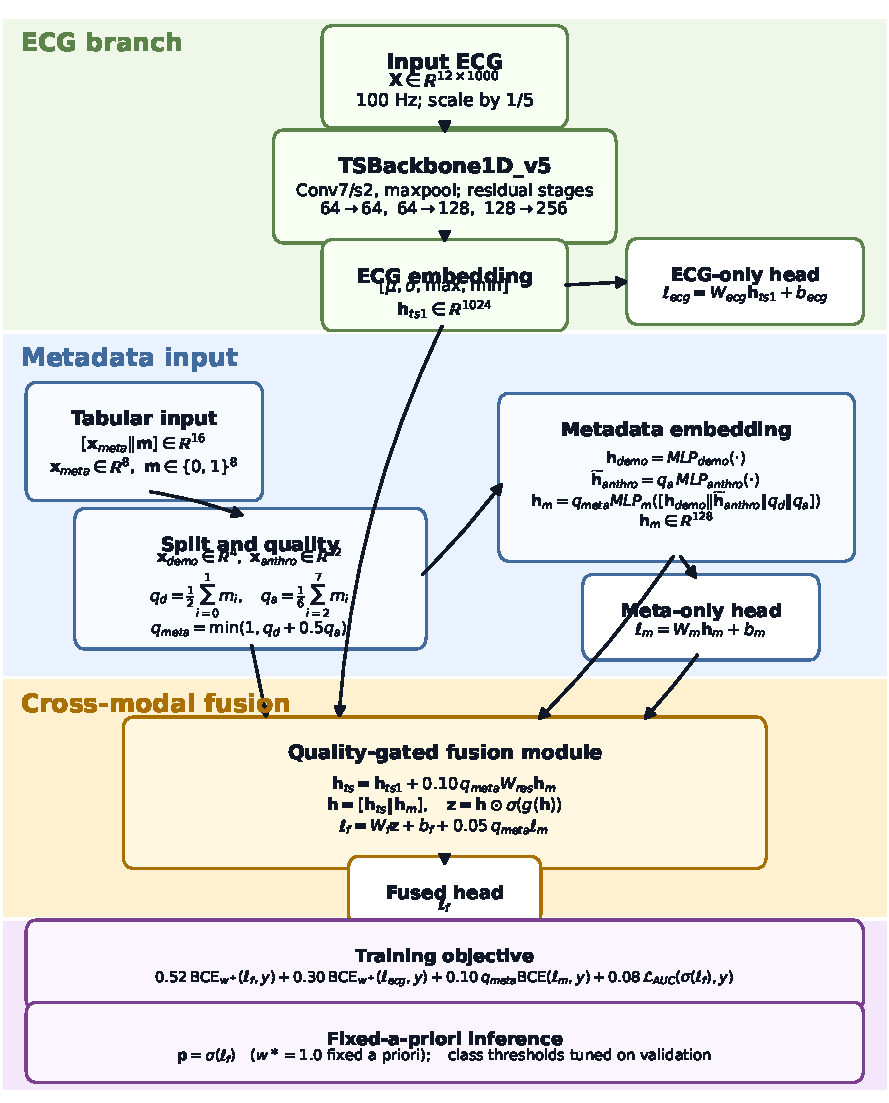
\includegraphics[width=\linewidth]{figures/fig1_architecture.pdf}
\caption{\textbf{EZNX-ATLAS-A architecture.} The 1D residual ECG backbone emits a 1024-dim temporal-statistics embedding $\mathbf{h}_{\mathrm{ts1}}$. A dual demographic/anthropometric MLP stack produces $\mathbf{h}_{\mathrm{m}}\in\mathbb{R}^{128}$, scaled by an explicit availability score $q_{\mathrm{meta}}$. One zero-initialised $1024\times128$ residual projection ($\mathbf{W}_{\mathrm{res}}$) softly biases the ECG embedding via residual injection (Eq.~\ref{eq:hts}); a second zero-initialised projection ($\mathbf{W}_{\mathrm{addon}}$) is instantiated exclusively for the E3 additive-injection ablation (Group~E). A GLU-inspired multiplicative gate fuses the concatenated embeddings. Three classification heads (fused, ECG-only, meta-only) enable multi-loss training; inference uses the fused-branch outputs ($w^{\ast}{=}1.0$ fixed a priori in all runs). Table~\ref{tab:hparams} reports the matched parameter budget (3.95\,M) and the archived compute provenance.}
\label{fig:arch}
\end{figure}

\subsection{ECG branch: TSBackbone1D\_v5}
An initial Conv1D ($k{=}7$, $s{=}2$, $p{=}3$, $12{\to}64$) with BatchNorm and ReLU is followed by MaxPool ($k{=}3$, $s{=}2$, $p{=}1$). Three residual stages, each with two residual blocks, implement the channel schedule $64{\to}64$ (stride 1), $64{\to}128$ (stride 2), $128{\to}256$ (stride 2), giving an output of shape $256\times T'$ with $T'{=}63$ for $T{=}1000$. A \emph{Temporal Statistics Pool} concatenates mean, standard deviation, max, and min over time:
\begin{equation}
\mathbf{h}_{\mathrm{ts1}}
= \bigl[\,\mu(\mathbf{F}),\ \sigma(\mathbf{F}),\ \max(\mathbf{F}),\ \min(\mathbf{F})\,\bigr]
\in \mathbb{R}^{1024}, \qquad \mathbf{F}\in\mathbb{R}^{256\times T'}.
\end{equation}

\subsection{Dual metadata encoder}
The loader returns the 8-dim tabular vector in Eq.~\eqref{eq:xmeta} together with its 8-dim availability mask $\mathbf{m}$. Each branch receives its feature slice concatenated with the corresponding mask slice, yielding a 4-dim demographic input (2 values~$+$~2 availability bits) and a 12-dim anthropometric input (6 values~$+$~6 availability bits):
\begin{align}
\mathbf{h}_{\mathrm{demo}}   &= \mathrm{MLP}_{\mathrm{demo}}(\mathbf{x}_{\mathrm{demo}}):\ \mathbb{R}^{4}\to\mathbb{R}^{64}\to\mathbb{R}^{64}\to\mathbb{R}^{64}, \\
\mathbf{h}_{\mathrm{anthro}} &= \mathrm{MLP}_{\mathrm{anthro}}(\mathbf{x}_{\mathrm{anthro}}):\ \mathbb{R}^{12}\to\mathbb{R}^{96}\to\mathbb{R}^{96}\to\mathbb{R}^{64}.
\end{align}
Each intermediate linear layer uses ReLU, BatchNorm, and 10\% Dropout; the final linear layer uses ReLU only.

\subsection{Availability-aware quality score}
We define per-block availability scores and an aggregate metadata-quality score:
\begin{equation}\label{eq:qmeta}
q_{d} = \tfrac{1}{2}\sum_{i=0}^{1} m_i, \qquad
q_{a} = \tfrac{1}{6}\sum_{i=2}^{7} m_i, \qquad
q_{\mathrm{meta}} = \min\!\bigl(1,\ q_{d} + 0.5\,q_{a}\bigr).
\end{equation}
In the working index, sex is always observed and age is observed for 98.7\% of records, so $q_d$ is usually 1, can drop to 0.5 when age is missing, and reaches 0 only in the theoretical edge case where both are unavailable (not observed in PTB-XL). Consequently, $q_{\mathrm{meta}} = \min(1,\,q_d + 0.5\,q_a) = 1$ for virtually all records in the \texttt{demo} and \texttt{demo+anthro} conditions (since $q_d{=}1$ implies $q_d + 0.5\,q_a \geq 1$). Graceful degradation under anthropometric missingness is therefore driven primarily by the explicit missingness flags ($m_h, m_w, m_{\mathrm{bmi}}$) in $\mathbf{x}_{\mathrm{meta}}$ and by sample meta-dropout; $q_{\mathrm{meta}}$ scaling provides the hard gate between the \texttt{none} variant ($q_{\mathrm{meta}}{=}0$) and any variant with demographics present ($q_{\mathrm{meta}}{=}1$).

\subsection{Meta-fusion MLP with sample meta-dropout}
Concatenation of the encoder outputs with the two availability scalars produces:
\begin{equation}\label{eq:hm}
\begin{aligned}
\widetilde{\mathbf{h}}_{\mathrm{anthro}} &= q_a\,\mathbf{h}_{\mathrm{anthro}},\\
\mathbf{u}_{\mathrm{m}}&=[\mathbf{h}_{\mathrm{demo}}\Vert\widetilde{\mathbf{h}}_{\mathrm{anthro}}\Vert q_d\Vert q_a]\in\mathbb{R}^{130},\\
\mathbf{h}_{\mathrm{m}}&=q_{\mathrm{meta}}\,\mathrm{MLP}_{\mathrm{m}}(\mathbf{u}_{\mathrm{m}})\in\mathbb{R}^{128}.
\end{aligned}
\end{equation}
During training with probability $p{=}0.10$, the entire pre-quality embedding is zeroed for the sample (\emph{sample meta-dropout}); at inference the dropout is disabled and $q_{\mathrm{meta}}$ scaling is applied.

\subsection{Residual injection}
\begin{equation}\label{eq:hts}
\mathbf{h}_{\mathrm{ts}} \;=\; \mathbf{h}_{\mathrm{ts1}}
  + 0.10\,q_{\mathrm{meta}}\,\mathbf{W}_{\mathrm{res}}\,\mathbf{h}_{\mathrm{m}},\qquad
\mathbf{W}_{\mathrm{res}}\in\mathbb{R}^{1024\times 128},\;\mathbf{W}_{\mathrm{res}}\leftarrow\mathbf{0}\text{ at init.}
\end{equation}
The projection $\mathbf{W}_{\mathrm{res}}$ is zero-initialised, making the injection path neutral at initialisation. A second independent zero-initialised projection $\mathbf{W}_{\mathrm{addon}}\in\mathbb{R}^{1024\times 128}$ is instantiated exclusively for the E3 additive-injection ablation (Group~E; Section~\ref{sec:sensitivity}) and is inert in the standard architecture (it receives zero gradient and remains at zero throughout standard-mode training). Because $\mathbf{h}_{\mathrm{m}}$ is itself scaled by $q_{\mathrm{meta}}$ (Eq.~\eqref{eq:hm}), the effective attenuation of the residual path is $q_{\mathrm{meta}}^{2}$, aggressively suppressing metadata-to-ECG cross-talk at partial availability.

\subsection{GLU-inspired fusion gate}
The gate applies element-wise multiplication to the full concatenated embedding (gating applied to the full 1152-dim concatenation without the feature splitting of the original GLU of~\cite{Dauphin2017}):
\begin{equation}
\mathbf{h} = [\mathbf{h}_{\mathrm{ts}}\Vert \mathbf{h}_{\mathrm{m}}]\in\mathbb{R}^{1152}, \qquad
\mathbf{z} = \mathbf{h} \odot \sigma\!\bigl(\mathrm{Linear}_2(\mathrm{ReLU}(\mathrm{Linear}_1(\mathbf{h})))\bigr)\in\mathbb{R}^{1152}.
\end{equation}

\subsection{Three heads with meta-correction}
\begin{align}
\bm{\ell}_{\mathrm{ecg}}   &= \mathbf{W}_{\mathrm{ecg}}\,\mathbf{h}_{\mathrm{ts1}} + \mathbf{b}_{\mathrm{ecg}}, \\
\bm{\ell}_{\mathrm{meta}}  &= \mathbf{W}_{\mathrm{meta}}\,\mathbf{h}_{\mathrm{m}} + \mathbf{b}_{\mathrm{meta}}, \\
\bm{\ell}_{\mathrm{fused}} &= \mathbf{W}_{\mathrm{fused}}\,\mathbf{z} + \mathbf{b}_{\mathrm{fused}} + 0.05\,q_{\mathrm{meta}}\,\bm{\ell}_{\mathrm{meta}}. \label{eq:headfused}
\end{align}
$\bm{\ell}_{\mathrm{ecg}}$ is computed on $\mathbf{h}_{\mathrm{ts1}}$ \emph{before} the residual injection in Eq.~\eqref{eq:hts}, preserving a strictly unimodal ECG branch. The $0.05\,q_{\mathrm{meta}}$ term in Eq.~\eqref{eq:headfused} provides a small direct metadata-logit correction to the fused head, gated by availability; at $q_{\mathrm{meta}}{=}0$ the fused head reduces to $\mathbf{W}_{\mathrm{fused}}\,\mathbf{z}+\mathbf{b}_{\mathrm{fused}}$ alone.

\subsection{Parameter budget}
The total is 3.95\,M trainable parameters: 0.96\,M in the ECG backbone, 0.06\,M in the dual metadata encoders and metadata-fusion MLP, 2.66\,M in the GLU fusion gate, 0.26\,M in the two metadata-to-ECG residual projections ($\mathbf{W}_{\mathrm{res}}$, active in the standard architecture, and $\mathbf{W}_{\mathrm{addon}}$, active in the E3 additive-injection ablation only; each $\mathbb{R}^{1024\times128}$, both zero-initialised), and 11.5\,k in the three classification heads. The GLU gate accounts for about 67\% of trainable parameters.

% =============================================================
\section{Training Protocol and Experimental Design}\label{sec:protocol}
% =============================================================

\subsection{Composite multi-task loss}
We minimise
\begin{equation}
\begin{aligned}
\mathcal{L}={}&0.52\,\mathrm{BCE}_{\mathbf{w}^{+}}\!(\bm{\ell}_{\mathrm{fused}},\mathbf{y})
 +0.30\,\mathrm{BCE}_{\mathbf{w}^{+}}\!(\bm{\ell}_{\mathrm{ecg}},\mathbf{y})\\
&+0.10\,q_{\mathrm{meta}}\,\mathrm{BCE}\!(\bm{\ell}_{\mathrm{meta}},\mathbf{y})
 +0.08\,\mathcal{L}_{\mathrm{AUC}}\!(\sigma(\bm{\ell}_{\mathrm{fused}}),\mathbf{y}),
\end{aligned}
\end{equation}
where $\mathrm{BCE}_{\mathbf{w}^{+}}$ is weighted multi-label binary cross-entropy with class weights from Eq.~\eqref{eq:posweights} and $\mathcal{L}_{\mathrm{AUC}}$ is an unsquared hinge AUC surrogate pooling all positive/negative label positions across the mini-batch.

\subsection{Optimiser and schedule}
AdamW with learning rate $10^{-3}$, weight decay $5{\times}10^{-4}$; CosineAnnealingWarmRestarts scheduler with $T_0{=}10$, $T_{\mathrm{mult}}{=}2$ (with $T_0{=}10$ matching the epoch budget, the schedule executes one complete cosine cycle and no warm restart is triggered); batch size 32, gradient accumulation 2 (effective batch 64); gradient clipping at $\Vert\nabla\Vert_{2}{\leq}1.0$; 10 epochs. The saved checkpoint is the epoch with the highest validation macro-AUC of the fused branch (with $w^{\ast}{=}1.0$ fixed). Operating thresholds are tuned per class on validation by maximising $F_{1}$ over 61 thresholds from 0.05 to 0.95.

\subsection{Fixed-a-priori inference}
Because $w^{\ast}{=}1.0$ is fixed \emph{a priori} according to the pre-declared analysis plan, per-class probabilities are computed directly from the fused branch:
\begin{equation}
\mathbf{p}(\mathbf{x}) = \sigma(\bm{\ell}_{\mathrm{fused}}).
\end{equation}
This is the $w^{\ast}{=}1.0$ special case of a fused/ECG convex blend, so no blend-weight grid search is performed; the fused head is used directly for all test predictions.

\subsection{Ablation variants}
We train three variants that differ \emph{only} in the metadata input:
\begin{description}[leftmargin=1.5em, style=sameline, font=\normalfont]
\item[\texttt{none}] $\mathbf{x}_{\mathrm{meta}}{\leftarrow}\mathbf{0}$, $\mathbf{m}{\leftarrow}\mathbf{0}$; $q_{\mathrm{meta}}{=}0$ and the metadata embedding is nulled after quality scaling.
\item[\texttt{demo}] age and sex are retained; height, weight, BMI values set to 0, their missingness indicators set to 1, and all anthropometric/missingness masks set to 0.
\item[\texttt{demo+anthro}] full 8-dim $\mathbf{x}_{\mathrm{meta}}$ as in Eq.~\eqref{eq:xmeta}.
\end{description}

\subsection{Seeds, runs, compute}
The full training campaign is organised in \textbf{six experimental groups (A--F)} totalling \textbf{250 unique runs} (270 seed-variant descriptors, of which 20 are shared between groups):

{\sloppy
\begin{description}[leftmargin=1.5em, style=sameline, font=\normalfont]
\item[\textbf{Group A} (primary confirmatory, 60 runs).] Three metadata variants (\texttt{none}, \texttt{demo}, \texttt{demo+anthro}) $\times$ \textbf{20 seeds} $\mathcal{S}{=}\{2024,\ldots,2043\}$, test fold 10, val fold 9. Python, NumPy, and PyTorch are each re-seeded at the start of every run; the random state is re-initialised immediately before \texttt{DataLoader} construction (after all index and split computations), so that within-seed batch ordering and augmentation trajectories are identical across the three variants for the same seed. In the \texttt{none} variant, $q_{\mathrm{meta}}{=}0$ nulls all metadata contributions; the metadata encoder parameters receive no gradient and remain at their random initialisation throughout training. Wall-clock time totalled 48.2\,h (median 43.8\,min/run; range $[43.1, 303.5]$\,min, the high value reflecting a transient CPU throttle at epoch~5 with no effect on convergence; the outlier run's final test macro-AUC is within the inter-seed standard deviation of its variant, as confirmed by its seed-level JSON record).
\item[\textbf{Group B} (exploratory, 30 unique runs).] Three non-reference \texttt{meta\_hid} values $\{32,64,256\}$ $\times$ 10 seeds, \texttt{demo+anthro} condition; reference $\texttt{meta\_hid}{=}128$ shares seeds with Group~A. Note: \texttt{meta\_hid} controls both projection and gate hidden dimensions (entangled).
\item[\textbf{Group C} (exploratory, 40 unique runs).] Four non-reference $\lambda_{\mathrm{LAUC}}$ values $\{0.00,0.04,0.12,0.16\}$ $\times$ 10 seeds; reference $\lambda{=}0.08$ shares seeds with Group~A. Note: $w_{\mathrm{fused}}{=}\max(0,\,0.60{-}\lambda_{\mathrm{LAUC}})$, so both weights change together. Additionally, the code normalises all four loss weights by their sum $(\texttt{total\_w})$ to ensure a bounded effective loss; for the values tested, $\texttt{total\_w}$ ranges from $0.98$ ($\lambda{=}0.16$) to $1.00$ ($\lambda{=}0.08$), making the renormalisation effect marginal but non-zero.
\item[\textbf{Group D} (exploratory, 20 unique runs).] Augmentation ablation: standard (\texttt{aug}, reference, 20 seeds $\mathcal{S}{=}\{2024,\ldots,2043\}$ shared with Group~A) vs.\ no-augmentation (\texttt{noaug}, 20 seeds $\mathcal{S}{=}\{2024,\ldots,2043\}$). The 20 noaug runs are the unique Group~D contribution; the aug reference is drawn from Group~A.
\item[\textbf{Group E} (exploratory, 80 runs).] Eight architectural ablations (E1--E8) $\times$ 10 seeds: meta-only fusion (E1), concatenation without gate (E2), additive injection without gate (E3), ReLU gate (E4), no residual injection (E5), availability signal disabled / $q{=}1$ always (E6), no feature dropout (E7), zero-metadata training / \texttt{trainmask} (E8).
\item[\textbf{Group F} (multi-split absolute-performance check, 20 runs).] Four alternative fold pairs (test/val: 2/3, 3/4, 7/8, 8/9) $\times$ 5 seeds, \texttt{demo+anthro} condition. No statistical test across the 20 runs as if independent (pre-declared); analysis unit is the fold.
\end{description}}%end \sloppy

The choice of 20 seeds for Group~A is a principled compromise between statistical resolution and the CPU-only computational budget. The paired Wilcoxon test at $n{=}20$ provides a minimum attainable exact $p$-value of approximately $0.000002$ ($= 2/2^{20} \approx 1.9\times10^{-6}$), enabling detection of small effects such as the demographic-only gain of $\Delta{=}+0.0007$ macro-AUC. Twenty seeds is above the modal practice in supervised deep learning evaluation, where three to five seeds are commonly reported~\cite{Bouthillier2021,Dodge2019}, and provides adequate power for the effect sizes observed here ($d_{\mathrm{z}}{=}0.64$ for \texttt{demo}$-$\texttt{none}; $d_{\mathrm{z}}{=}1.65$ for \texttt{demo+anthro}$-$\texttt{none}).

Table~\ref{tab:run_ledger} provides a complete run-accounting ledger to support reproducibility auditing. The ``Unique runs'' column counts runs not present in any other group; shared reference seeds are listed in the ``Reference source'' column.

\begin{table}[H]
\caption{Run-accounting ledger for the 250-run campaign ($\mathcal{S}_{10}{=}\{2024,\ldots,2033\}$; $\mathcal{S}_{20}{=}\{2024,\ldots,2043\}$). Groups~B, C, and~E share 10 Group~A \texttt{demo+anthro} seeds as their reference, yielding 20 shared descriptors in the 270-descriptor total.}\label{tab:run_ledger}
\small\centering
\begin{tabular}{llcccc}
\toprule
\textbf{Grp} & \textbf{Description} & \textbf{Seeds} & \textbf{Unique} & \textbf{$n$} & \textbf{Role} \\
\midrule
A & 3 variants (none/demo/da) & $\mathcal{S}_{20}$ ea. & 60 & 20 & Confirmatory \\
B & 3 meta\_hid values; ref shared w/A & $\mathcal{S}_{10}$ ea. & 30 & 10 & Exploratory \\
C & 4 $\lambda_{\mathrm{LAUC}}$ values; ref shared w/A & $\mathcal{S}_{10}$ ea. & 40 & 10 & Exploratory \\
D & noaug; aug ref from A & $\mathcal{S}_{20}$ & 20 & 20 & Exploratory \\
E & 8 arch ablations; std ref from A & $\mathcal{S}_{10}$ ea. & 80 & 10 & Exploratory \\
F & 4 alt.\ fold pairs, \texttt{da} only & 5 ea. & 20 & 5/fold & Gen.\ check \\
\midrule
\multicolumn{3}{l}{\textbf{Total unique runs}} & \textbf{250} & & \\
\multicolumn{3}{l}{\textbf{Total descriptors (incl.\ shared)}} & \textbf{270} & & \\
\bottomrule
\end{tabular}
\end{table}

\subsection{Statistical analysis}
We report macro-AUC and macro-$F_1^{\ast}$ as mean $\pm$ standard deviation across seeds. Marginal 95\% percentile bootstrap CIs are obtained by resampling the 20 seed-level values 10{,}000 times; paired-difference CIs are obtained by resampling the 20 seed-matched differences. Pairwise inference uses exact two-sided paired Wilcoxon signed-rank tests~\cite{Hollander2014} on seed-matched variant differences, implemented with \texttt{scipy.stats.wilcoxon} (SciPy 1.16.3, \texttt{zero\_method="wilcox"}, \texttt{correction=False}, exact $p$-values for $n{\leq}25$). We report Cohen's $d_{\mathrm{z}}$ as the main descriptive paired effect size and Hedges-corrected $g_{\mathrm{z}}$ as a small-sample companion.

\textbf{BH-FDR family (Group~A, confirmatory).} Benjamini--Hochberg FDR control at $q{=}0.05$ is applied across the \textbf{pre-specified 3-test family}: the three pairwise macro-AUC contrasts in Group~A (none vs.\ demo; none vs.\ demo+anthro; demo vs.\ demo+anthro). With $n{=}20$, the attainable raw two-sided $p$-values are discrete; the minimum attainable exact Wilcoxon $p$ at $n{=}20$ is approximately $0.000002$ ($= 2/2^{20} \approx 1.9\times10^{-6}$, achieved when all 20 signed-rank sums equal 0 or 210).

\textbf{Exploratory groups (B, C, D, E).} Results for Groups~B, C, D, and E are exploratory. Wilcoxon $p$-values are reported for descriptive purposes without multiple-comparison correction; no confirmatory inference should be drawn from these values.

\textbf{Secondary per-class sub-family (DA$-$NONE, Table~\ref{tab:perclass}).} As a secondary, post-hoc analysis, BH-FDR correction is additionally applied within the 5-test sub-family of per-class DA$-$NONE Wilcoxon tests (NORM, MI, STTC, CD, HYP). This sub-family was not pre-specified and serves descriptive purposes only. Per-class tests for the \texttt{demo}$-$\texttt{none} contrast are exploratory and reported as raw $p$-values only.

\textbf{Group~F (multi-split absolute-performance check).} No statistical test across the 20 Group~F runs as if independent. Analysis is at the fold level (4 units); the primary quantity is the inter-fold macro-AUC range.

Decision thresholds are tuned per class on fold~9 and fixed for fold~10; reported $p$-values are therefore conditional on this validation-based model-selection protocol.

\subsection{Methodological contribution and fit with Mathematics}
The seed-matched paired-Wilcoxon measurement pipeline introduced here is a generalisable statistical framework for multimodal-ML ablations, and constitutes the primary methodological contribution of this work to the mathematical sciences. For each seed $s$ and variant $V_k$, one trains to obtain a scalar evaluation metric $r_{k,s}$. Pairwise incremental effects are estimated as $\delta_{jk,s} = r_{j,s} - r_{k,s}$. Inference proceeds by applying the exact two-sided Wilcoxon signed-rank test (a distribution-free rank test on signed differences), BH-FDR correction over the pre-specified confirmatory test family (controlling the expected proportion of false discoveries among rejected hypotheses), and percentile bootstrap confidence intervals on the seed-matched differences. Effect sizes are reported as Cohen's $d_{\mathrm{z}}$ with Hedges' small-sample correction $g_{\mathrm{z}}$. Exploratory groups report raw $p$-values descriptively without FDR correction. The framework provides a principled approach to the multiple-comparison problem in deep learning ablation studies, separating a pre-specified confirmatory family (3-test BH-FDR) from exploratory nominal $p$-values, and quantifying incremental contributions with calibrated uncertainty. It applies to any setting satisfying three conditions: (i) a baseline model can be paired with an augmented variant across the same random seeds; (ii) the number of seeds is small (say, $n \in [5, 20]$); and (iii) one seeks calibrated inference about the incremental contribution of an additional input modality or component.

% =============================================================
\section{Results}\label{sec:results}
% =============================================================

\subsection{Aggregate performance}
All reported $p$-values are conditional on the validation-based model-selection protocol.
Table~\ref{tab:main} reports macro-AUC and macro-$F_1^{\ast}$ for each variant as mean $\pm$ standard deviation across 20 seeds, together with 95\% bootstrap CIs and paired Wilcoxon $p$-values. The \texttt{demo+anthro} variant reaches $0.9289 \pm 0.0013$ macro-AUC on fold-10, numerically close to the 10-fold CV mean of the xresnet1d101 benchmark of~\cite{Strodthoff2021} ($0.928 \pm 0.005$; direct comparison is limited as our evaluation uses fold-10 alone, and Group~F descriptively shows that absolute demo+anthro AUC was lower on fold~10 than on four alternative folds, consistent with fold-level difficulty variation).

A key finding is that \textbf{both demographic-only and full-metadata gains are statistically significant} across 20 paired seeds. The \texttt{demo}$-$\texttt{none} difference is $+0.0007 \pm 0.0002\ (\mathrm{SEM})$ macro-AUC with a 95\% paired bootstrap CI of $[0.0002, 0.0011]$ ($p_{\mathrm{raw}}{=}0.0094$, $p_{\mathrm{BH}}{\approx}0.009$, $d_{\mathrm{z}}{=}0.64$, $g_{\mathrm{z}}{=}0.61$; 16 of 20 paired seed differences positive). The \texttt{demo+anthro}$-$\texttt{none} contrast yields $+0.0019 \pm 0.0003\ (\mathrm{SEM})$ macro-AUC with a 95\% paired bootstrap CI of $[0.0014, 0.0023]$ ($p_{\mathrm{raw}}{\approx}0.00001$, $p_{\mathrm{BH}}{<}0.001$, $d_{\mathrm{z}}{=}1.65$, $g_{\mathrm{z}}{=}1.58$; 19 of 20 differences positive). The demographic gain is real but smaller than the anthropometric component; the incremental anthropometric step (\texttt{demo+anthro}$-$\texttt{demo}) is itself significant ($+0.0012 \pm 0.0003\ (\mathrm{SEM})$, $p_{\mathrm{BH}}{\approx}0.001$, $d_{\mathrm{z}}{=}0.95$). These results should be read as protocol-specific measurements rather than as large clinical effect sizes.

\subsection{Per-class decomposition}
Table~\ref{tab:perclass} and Figs.~\ref{fig:delta} and \ref{fig:heat} report class-wise AUC and the corresponding $\Delta$-AUC for the \texttt{demo+anthro} minus \texttt{none} contrast. With 20 seeds and BH-FDR correction, \textbf{three classes reach significance}: \textbf{NORM} ($+0.0016$, $p_{\mathrm{BH}}{<}0.0001$), \textbf{MI} ($+0.0058$, $p_{\mathrm{BH}}{<}0.0001$), and \textbf{STTC} ($+0.0018$, $p_{\mathrm{BH}}{=}0.00035$). The MI effect has the largest absolute delta ($+0.0058$) and a strong $d_{\mathrm{z}}{=}2.26$. CD shows a negligible shift ($-0.0003$, $p_{\mathrm{BH}}{=}0.648$). \textbf{HYP shows no statistically significant gain} ($+0.0004$, $p_{\mathrm{BH}}{=}0.648$); we return to this HYP pattern in Section~\ref{sec:discussion}.

For the \texttt{demo}$-$\texttt{none} contrast, exploratory per-class Wilcoxon tests identify significance for NORM ($+0.0006$, $p_{\mathrm{raw}}{=}0.006$) and MI ($+0.0020$, $p_{\mathrm{raw}}{=}0.003$), indicating that even demographic variables alone carry a per-class signal in these two morphology-rich classes. These per-class tests are not in the pre-specified BH-FDR family and are reported descriptively.

\subsection{Training dynamics}
Figure~\ref{fig:curves} shows the validation macro-AUC trajectory across 10 training epochs for all three variants, displayed as mean~$\pm$~standard deviation across all 20 seeds. The cross-seed SD narrows from $0.008$--$0.010$ at epoch~1 to ${\approx}0.001$ at epoch~10. All three variants converge to near-final performance by epoch~7--8. The final-epoch means and SDs are: \texttt{none} $0.9320\pm0.0012$, \texttt{demo} $0.9323\pm0.0008$, \texttt{demo+anthro} $0.9330\pm0.0012$.

\subsection{Missingness robustness}
Figure~\ref{fig:missing} shows inference-time macro-AUC under synthetic anthropometric masking. The empirical masking curve is evaluated on the \texttt{demo+anthro} variant across \textbf{10 seeds} (seeds 2024--2033; the pre-declared analysis plan specified 20 seeds---this deviation was made for computational efficiency; see Limitation~8); the \texttt{none} and \texttt{demo} variant traces are included as structural reference baselines (they are immune to anthropometric masking by construction: \texttt{none} receives no metadata, and \texttt{demo} contains no anthropometric fields to mask). At each masking rate $\rho \in \{0, 0.25, 0.5, 0.75, 1.0\}$, each of the three anthropometric fields (height$_z$, weight$_z$, BMI$_z$) is independently zeroed with probability $\rho$ at inference time; the three corresponding missingness indicators ($m_h$, $m_w$, $m_{\mathrm{bmi}}$) and availability mask bits are updated consistently. Demographic fields (age$_z$, sex01) are never masked and remain available throughout. Note that BMI is derived from height and weight, so independent masking of the three fields can produce states where BMI is masked while only one of height or weight is masked; this is treated as a maximal stress test rather than a physiologically realistic dropout scenario, and the scenario was not explored under joint anthropometric-field masking. The stress-test curve remains stable: full anthropometric masking costs only $\approx 0.0014$ macro-AUC relative to the unmasked model (Panel~A, $\Delta$ annotation). At $\rho{=}1.0$ the \texttt{demo+anthro} model converges to the \texttt{demo} baseline (difference $-0.00018$, less than $\frac{1}{6}$ cross-seed SD) and remains $+0.00047$ above the \texttt{none} baseline. Panel~B clarifies that the \texttt{none} variant is immune by construction (flat), while \texttt{demo} shows minimal drift ($<0.0001$). This demonstrates graceful degradation under deployment-time field dropout.

\subsection{Seed distribution and fused-branch gain}
Figure~\ref{fig:blend} shows the distribution of test macro-AUC across all 20 seeds for each variant. The \texttt{demo+anthro} violins are shifted upward relative to \texttt{none} and \texttt{demo}, with minimal within-variant variance ($\mathrm{SD}{\leq}0.0013$). The significance brackets confirm the two BH-FDR confirmatory contrasts (Section~\ref{sec:protocol}). Across seeds, the fused head consistently outperforms the ECG-only auxiliary head for \texttt{demo+anthro}: the $\mathrm{AUC}_{\mathrm{fused}} - \mathrm{AUC}_{\mathrm{ecg}}$ gap is positive for \textbf{all 20 of 20 seeds} (median $+0.0016$; Panel~B of Fig.~\ref{fig:blend}; note that the ECG auxiliary head is trained jointly inside the multimodal model, not as an independent ECG-only baseline---the \texttt{none} variant serves as the independent ECG-only reference; note also that the fused head is trained with both BCE and AUC surrogate losses, while the ECG auxiliary head is trained with BCE only, so the fused--ECG gap partly reflects this training asymmetry in addition to the metadata contribution), whereas for \texttt{none} and \texttt{demo} this gap is centred near zero (8/20 and 16/20 positive; medians $-0.0001$ and $+0.0003$ respectively). This is consistent with $w^{\ast}{=}1.0$ fixed a priori: when metadata help, the fused branch captures the gain.

\subsection{Comparison with prior work}
Tables~\ref{tab:prior_a}--\ref{tab:prior_b} position EZNX-ATLAS-A through a comparability audit rather than within a heterogeneous leaderboard. Our direct numerical comparator is the canonical PTB-XL super-diagnostic benchmark of Strodthoff~\textit{et al.}~\cite{Strodthoff2021}: the \texttt{none} variant lies approximately $0.001$ macro-AUC below the 10-fold CV mean ($0.9271$ vs.\ $0.928$; comparison is indicative as our evaluation uses fold-10 alone, and Group~F descriptively shows that absolute macro-AUC varied across splits, with fold~10 below the inter-fold range) while using a substantially smaller trainable model. The self-supervised and multimodal papers listed in Table~\ref{tab:prior_b} address neighbouring questions, but their task definitions, datasets, or metadata modalities differ from our seed-matched PTB-XL demographic/anthropometric ablation.

\subsection{Architectural diagnostics and sensitivity ablations}
\label{sec:sensitivity}
With $w^{\ast}{=}1.0$ fixed a priori, test predictions are those of the fused head alone for all runs.

\paragraph{Groups B and C: hyperparameter sensitivity (exploratory).}
Table~\ref{tab:sensitivity} reports multi-seed (10 seeds) exploratory sensitivity results for Groups~B and C. Group~B tests three non-reference \texttt{meta\_hid} values $\{32, 64, 256\}$ against the reference (128, shared with Group~A); all Wilcoxon $p{>}0.32$ versus the reference, spanning the macro-AUC range $0.9285$--$0.9296$ with overlapping intervals. Note that \texttt{meta\_hid} controls both the projection dimension and the gate hidden dimension simultaneously (entangled); varying it does not isolate a single architectural degree of freedom. Group~C tests four non-reference $\lambda_{\mathrm{LAUC}}$ values $\{0.00, 0.04, 0.12, 0.16\}$ against the reference (0.08, shared with Group~A); all variants are within the noise of the reference, with $p$-values ranging from $0.557$ to $0.695$. Note that $w_{\mathrm{fused}} = \max(0, 0.60 - \lambda_{\mathrm{LAUC}})$, so the two loss weights change simultaneously when $\lambda_{\mathrm{LAUC}}$ is varied. These results show no detectable sensitivity under this exploratory design, rather than identifying an optimal configuration; no BH-FDR correction is applied to exploratory groups.

\begin{table}[H]
\caption{Exploratory sensitivity: fusion capacity (Group~B, \texttt{meta\_hid} controls projection and gate hidden dim jointly) and LAUC-BCE balance (Group~C; $w_{\mathrm{fused}} = \max(0,0.60-\lambda_{\mathrm{LAUC}})$, both weights change simultaneously). \texttt{demo+anthro} condition, 10 seeds. $\dagger$ = default value. Wilcoxon $p$-values ($n{=}10$, exact two-sided) are reported descriptively; no FDR correction is applied to exploratory groups.}\label{tab:sensitivity}
\small\centering
\begin{tabular}{llcc}
\toprule
\textbf{Group} & \textbf{Parameter / Value} & \textbf{Macro-AUC (mean$\pm$SD)} & \textbf{Wilcoxon $p$ vs.\ ref} \\
\midrule
B & \texttt{meta\_hid} = 32  & $0.9285\pm0.0013$ & $0.322$ \\
B & \texttt{meta\_hid} = 64  & $0.9285\pm0.0014$ & $0.432$ \\
B & \texttt{meta\_hid} = 128$\dagger$ (ref) & $0.9289\pm0.0012$ & --- \\
B & \texttt{meta\_hid} = 256 & $0.9296\pm0.0010$ & $0.322$ \\
\midrule
C & $\lambda_{\mathrm{LAUC}} = 0.00$ & $0.9286\pm0.0017$ & $0.557$ \\
C & $\lambda_{\mathrm{LAUC}} = 0.04$ & $0.9291\pm0.0012$ & $0.695$ \\
C & $\lambda_{\mathrm{LAUC}} = 0.08\dagger$ (ref) & $0.9289\pm0.0012$ & --- \\
C & $\lambda_{\mathrm{LAUC}} = 0.12$ & $0.9288\pm0.0008$ & $0.625$ \\
C & $\lambda_{\mathrm{LAUC}} = 0.16$ & $0.9291\pm0.0008$ & $0.557$ \\
\bottomrule
\end{tabular}
\end{table}

\paragraph{Group D: augmentation ablation (exploratory).}
Training without stochastic augmentation (\texttt{noaug}) yields macro-AUC $0.9275{\pm}0.0012$ versus $0.9289{\pm}0.0012$ for the augmented reference ($\Delta{=}{-}0.0014$, nominal $p{=}0.002$, $r{=}0.725$, $n{=}20$; exploratory, no FDR correction applied). This is the only exploratory group to show a nominally significant difference from the reference configuration. The result suggests that the light augmentation block (Gaussian noise, temporal shift, amplitude jitter) contributes a measurable positive effect and should be treated as a factor to control and report rather than an optional add-on; confirmatory inference would require a pre-declared seed budget and BH-FDR correction.

\paragraph{Group E: architectural ablations (exploratory).}
Table~\ref{tab:group_e} reports macro-AUC for eight architectural ablations against the standard configuration (10 seeds each). Two extreme variants show catastrophic degradation: \textbf{E1 meta-only} ($0.6966{\pm}0.0021$, $p{=}0.002$, exploratory) suggests that the ECG signal is indispensable under this design, and \textbf{E8 trainmask} ($0.5046{\pm}0.0180$, $p{=}0.002$)---in which the model is trained with zeroed metadata and then evaluated with real metadata---is a distribution-shift negative control: training without the metadata pathway prevents its use at inference time. This result does not imply that metadata must generally be present during training; the \texttt{none} variant ($0.9271$ macro-AUC) demonstrates that ECG-only training without any metadata pathway is fully viable. All six remaining ablations (E2--E7) show macro-AUC within $\pm0.0004$ of the reference with $p{>}0.27$, indicating that the specific choice of fusion mechanism (concatenation, additive injection, GLU gate) and the inclusion of residual injection, availability signal, and feature dropout do not materially affect macro-AUC.

\begin{table}[H]
\caption{Architecture ablations (Group~E, exploratory). \texttt{demo+anthro} variant, 10 seeds ($\mathcal{S}_{10}{=}\{2024,\ldots,2033\}$). E8 (\texttt{trainmask}): standard architecture trained with $\mathbf{x}_{\mathrm{meta}}{=}\mathbf{0}$, $\mathbf{m}{=}\mathbf{0}$; evaluated with real metadata. Wilcoxon $p$-values ($n{=}10$, exact two-sided) vs.\ Standard reference (also 10 seeds, $\mathcal{S}_{10}$; the full 20-seed $\mathcal{S}_{20}$ statistics are reported in Table~\ref{tab:main}).}\label{tab:group_e}
\small\centering
\begin{tabular}{lcc}
\toprule
\textbf{Configuration} & \textbf{Macro-AUC (mean$\pm$SD)} & \textbf{Wilcoxon $p$} \\
\midrule
Standard (reference, Group~A) & $0.9289\pm0.0012$ & --- \\
E1: Meta-only fusion           & $0.6966\pm0.0021$ & $0.002$ \\
E2: Concatenation (no gate)    & $0.9290\pm0.0010$ & $0.922$ \\
E3: Additive injection (no gate) & $0.9290\pm0.0012$ & $0.846$ \\
E4: ReLU gate (no sigmoid)     & $0.9288\pm0.0014$ & $0.770$ \\
E5: No residual injection      & $0.9292\pm0.0012$ & $0.695$ \\
E6: No availability signal ($q{=}1$) & $0.9287\pm0.0013$ & $0.557$ \\
E7: No feature dropout         & $0.9293\pm0.0008$ & $0.275$ \\
E8: Trainmask (zero meta at training) & $0.5046\pm0.0180$ & $0.002$ \\
\bottomrule
\end{tabular}
\end{table}

\paragraph{Group F: multi-split absolute-performance check (descriptive).}
Table~\ref{tab:group_f} reports macro-AUC for the \texttt{demo+anthro} model on four alternative test folds (5 seeds each). The inter-fold range is $[0.9400, 0.9445]$, with a mean of $0.9425$ across the four folds. \textbf{Fold~10 (Group~A reference, $0.9289\pm0.0013$) lies below this range by 0.0111--0.0156 macro-AUC}, indicating that absolute performance varied across split definitions. Group~A absolute macro-AUC for the \texttt{demo+anthro} condition is therefore conditioned on a more challenging split; the within-fold paired variant comparisons (none vs.\ demo vs.\ demo+anthro) in Group~A are unaffected by this fold-level variation. \emph{Important caveat:} the metadata z-scoring and imputation index was constructed from folds 1--8 of the primary split. For all four Group~F alternative splits, the test folds (2, 3, 7, 8) were included in the original scaler; this normalization dependency means the absolute macro-AUC values in Table~\ref{tab:group_f} are not fully independent of the primary split's preprocessing and should be interpreted as descriptive only. Likewise, only the \texttt{demo+anthro} variant was evaluated on these alternative splits; the \texttt{none} and \texttt{demo} variants were not re-run, so within-fold paired gains cannot be assessed for Group~F.

\begin{table}[H]
\caption{Multi-split absolute-performance check (Group~F, descriptive only). \texttt{demo+anthro} model only, 5 seeds per split. Analysis unit: fold (4 units); no statistical test across the 20 runs as if independent. Absolute performance varied across split definitions; fold~10 had lower absolute macro-AUC than the four alternative test folds. \emph{Normalization caveat:} the metadata z-scoring index was built from folds~1--8 of the primary split; the Group~F test folds (2, 3, 7, 8) were part of this scaler and are therefore not fully independent of the primary preprocessing---treat all values as descriptive. The \texttt{none} and \texttt{demo} variants were not re-evaluated on these splits; within-fold metadata gains cannot be assessed. Group~A (fold~10) reference shown for comparison.}\label{tab:group_f}
\small\centering
\begin{tabular}{cclc}
\toprule
\textbf{Test fold} & \textbf{Val fold} & \textbf{$n$ seeds} & \textbf{Macro-AUC (mean$\pm$SD)} \\
\midrule
2 & 3 & 5 & $0.9422\pm0.0007$ \\
3 & 4 & 5 & $0.9400\pm0.0006$ \\
7 & 8 & 5 & $0.9434\pm0.0007$ \\
8 & 9 & 5 & $0.9445\pm0.0013$ \\
\midrule
10 (Group~A) & 9 & 20 & $0.9289\pm0.0013$ (reference) \\
\bottomrule
\multicolumn{4}{l}{\footnotesize Inter-fold range (folds 2,3,7,8): $[0.9400, 0.9445]$; mean: $0.9425$}\\
\end{tabular}
\end{table}

% =============================================================
\section{Discussion}\label{sec:discussion}
% =============================================================

\subsection{Q1 --- when do metadata help?}
Our 20-seed protocol yields a clear and nuanced answer. \textbf{Both demographic and anthropometric variables show statistically significant gains.} Demographics alone (age, sex) yield $\Delta{=}+0.0007$ macro-AUC ($p_{\mathrm{BH}}{\approx}0.009$, $d_{\mathrm{z}}{=}0.64$, $n_{\mathrm{pos}}{=}16/20$ seeds). This small but reproducible effect is consistent with the partial recoverability argument of Attia~\textit{et al.}~\cite{Attia2019AgeSex}: age and sex are substantially recoverable from the waveform (sex AUC 0.97, age MAE 6.9\,y), yet a residual increment not fully captured by the ECG-only model remains detectable with 20 paired seeds. The incremental anthropometric gain beyond demographics is larger and more significant ($\Delta{=}+0.0012$, $p_{\mathrm{BH}}{\approx}0.001$, $d_{\mathrm{z}}{=}0.95$): body-size variables provide complementary information not easily recoverable from the 12-lead waveform alone. Both effects remain small in absolute terms ($\Delta{<}0.002$ macro-AUC) and should be read as protocol-specific measurements rather than as clinically large effect sizes. No clinical decision benefit, calibration improvement, or net-reclassification gain is claimed; whether these AUC increments translate to any clinical utility requires prospective evaluation on held-out cohorts.

\subsection{Q2 --- which class benefits from which metadata? The MI/STTC/NORM finding}
With 20 seeds and BH-FDR correction, the class-wise effect of full metadata localises to three classes. \textbf{MI} shows the strongest effect ($+0.0058$, $p_{\mathrm{BH}}{<}0.0001$, $d_{\mathrm{z}}{=}2.26$), followed by \textbf{STTC} ($+0.0018$, $p_{\mathrm{BH}}{=}0.00035$) and \textbf{NORM} ($+0.0016$, $p_{\mathrm{BH}}{<}0.0001$). Exploratory per-class tests for the demographic-only contrast (\texttt{demo}$-$\texttt{none}) also identify nominal significance for NORM ($p_{\mathrm{raw}}{=}0.006$) and MI ($p_{\mathrm{raw}}{=}0.003$); these tests are not in any pre-specified BH-FDR family and are reported descriptively. This pattern suggests that age and sex supply a useful prior for morphology-sensitive classes even when anthropometrics are absent. Plausible but non-causal hypotheses include body-size-conditioned calibration of ST-segment amplitudes, Q-wave depth, and related markers for MI, and thoracic electrical property effects for STTC; these are associations consistent with the observed patterns, not causal attributions.

\subsection{The HYP paradox: no detectable gain at the superclass level}
Even with 20 seeds, \textbf{HYP shows no statistically significant gain} ($+0.0004$, $p_{\mathrm{BH}}{=}0.648$). This pattern is consistent with four explanatory hypotheses: (1) low HYP prevalence limits paired test power for a genuinely small effect; (2) the TSPool's $\max/\min$ voltage statistics already partially absorb body-habitus effects; (3) superclass heterogeneity dilutes a more specific LVH-related signal; and (4) HYP label noise in borderline cases attenuates any body-habitus signal. The non-significant HYP result with 20 seeds makes a large effect unlikely under this protocol, though smaller or subclass-specific effects (e.g., an LVH-specific signal beneath the superclass label) remain possible and were not tested here. Exploratory examination of the \texttt{demo}$-$\texttt{none} HYP test ($\Delta{=}+0.0015$, $p_{\mathrm{raw}}{=}0.048$) reveals a borderline positive demographic signal that does not pass the exploratory threshold of $p{<}0.01$ and is not sustained in the full-metadata DA$-$NONE contrast ($p_{\mathrm{BH}}{=}0.648$), consistent with the interpretation that anthropometric variables do not amplify the marginal demographic effect for HYP.

\subsection{CD: demographics and the confounding role of age}
The \texttt{demo} variant produces a slight negative trend in CD AUC ($-0.0011$, $p_{\mathrm{raw}}{=}0.123$, exploratory), but this does not survive BH-FDR correction at 20 seeds. This remains consistent with the age-as-confounder hypothesis: directly supplying age may shift the CD decision boundary, but the effect is not reproducibly negative. The \texttt{demo+anthro} CD delta is also non-significant ($-0.0003$, $p_{\mathrm{BH}}{=}0.648$).

\subsection{Q3 --- graceful degradation}
The availability-aware pathway---combining missingness indicators (Eq.~\eqref{eq:xmeta}), zero-initialised residual injection (Eq.~\eqref{eq:hts}), and sample meta-dropout during training---yields a model whose macro-AUC under full anthropometric suppression remains within $\approx 0.0014$ of the full unmasked variant (Fig.~\ref{fig:missing}), converging to the demographics-only baseline. In PTB-XL, $q_{\mathrm{meta}}$ saturates to 1 for nearly all records when age and sex are present (as in the \texttt{demo} and \texttt{demo+anthro} conditions); the primary graceful-degradation mechanism under anthropometric dropout is therefore \textbf{sample meta-dropout} (which trains the model to function without anthropometric inputs) and \textbf{median imputation} (which provides a neutral fallback value). The missingness indicators $m_h$, $m_w$, $m_{\mathrm{bmi}}$ contribute primarily when the corresponding field is present (their availability mask equals 1 when the field is observed, and 0 when the field is absent); they do not act as an explicit ``field is missing'' signal through the availability-gating pathway when a field is absent. $q_{\mathrm{meta}}$ acts mainly as a hard gate between the all-metadata and no-metadata conditions. This robustness is demonstrated under synthetic inference-time masking; generalisability to structurally missing data under MCAR, MAR, or MNAR mechanisms remains an open evaluation direction.

\subsection{Group D: augmentation should be controlled and reported}
The exploratory Group~D result ($\Delta{=}{-}0.0014$, nominal $p{=}0.002$, $n{=}20$, no FDR correction applied) reveals that the light stochastic augmentation block---Gaussian noise, temporal shift, and amplitude jitter---contributes a measurable positive effect. This nominally significant finding (the only such result among all exploratory groups) suggests that augmentation should be treated as a design factor to control and report rather than an optional add-on; confirmatory inference would require a pre-declared seed budget and BH-FDR correction.

\subsection{Q4 --- comparability of earlier multimodal gains}
Our 20-seed protocol reveals within-variant standard deviations of $0.0010$--$0.0013$ macro-AUC, of the same order as the measured between-variant effects. The audited literature does not provide a directly comparable PTB-XL experiment separating age/sex from height/weight/BMI with repeated seeds, paired tests, and missingness stress testing. We therefore position this paper as providing a narrow but statistically honest reproducibility baseline: $+0.0007$ from demographics and $+0.0019$ from full metadata, with class-resolved and missingness-audited evidence.

\subsection{Q5 --- architectural ablations: ECG is essential, gating is flexible}
Exploratory Group~E ablations (10 seeds, uncorrected) suggest two patterns. First, the ECG signal is indispensable: the meta-only variant (E1) collapses to $0.6966$ macro-AUC, far below any ECG-based variant in this study. Second, the specific fusion mechanism does not drive macro-AUC differences at this scale: all six mechanism variants (E2--E7) achieve $0.9287$--$0.9293$, within the noise of the standard configuration ($p{>}0.27$ in all cases). This is notable because E2 (simple concatenation) and E3 (additive injection) achieve performance comparable to the GLU gate, suggesting that the gate's added complexity is not necessary to capture the metadata signal at this effect magnitude. The E8 result ($0.5046$ macro-AUC) is a distribution-shift negative control: training with zeroed metadata and then evaluating with real metadata induces a severe train/inference distribution mismatch. This does not imply that metadata must generally be present during training; the \texttt{none} variant ($0.9271$ macro-AUC) demonstrates that ECG-only training without any metadata pathway remains fully competitive.

\subsection{Q6 --- fold-level variation: absolute performance varied across split definitions}
Group~F shows that the four alternative fold pairs (folds 2, 3, 7, 8 as test folds) all achieve macro-AUC in the range $[0.9400, 0.9445]$, substantially above fold~10 ($0.9289$). This $0.011$--$0.016$ gap is consistent with fold-level difficulty variation in stratified k-fold settings and indicates that absolute \texttt{demo+anthro} macro-AUC varied across the tested splits. The within-fold paired comparisons of Group~A are unaffected by this fold-level variation; the absolute difference should be noted when positioning fold-10 results relative to benchmarks evaluated on averaged or best-of-fold metrics. Two important limitations apply to Group~F: first, the metadata normalization index was built from folds 1--8 of the primary split, meaning the alternative test folds (2, 3, 7, 8) were included in the original scaler---these values should therefore be treated as descriptive rather than confirming a pattern independent of the primary preprocessing; second, because \texttt{none} and \texttt{demo} variants were not re-evaluated on the alternative splits, within-fold metadata gains cannot be assessed.

\subsection{Sensitivity ablations: no detectable sensitivity to hyperparameters}
The exploratory multi-seed sensitivity analyses (Groups~B and C, Section~\ref{sec:sensitivity}) are consistent with the reported results not being sensitive to a specific metadata hidden size or AUC-surrogate weight. All seven non-reference variants (three metaH, four lauc) show Wilcoxon $p{>}0.32$ against the standard configuration, with macro-AUC ranges spanning less than $0.0012$; no confirmatory inference is drawn from these exploratory results.

\subsection{Why small measured effects remain informative}
Reporting $+0.0007$ and $+0.0019$ macro-AUC gains is a refinement of the multimodal claim rather than a null result. The paired seed-level 95\% CIs are strictly positive for the full-metadata contrast ($[0.0014, 0.0023]$), supporting a reproducible directional effect without implying a large clinical effect size. The demographic-only CI ($[0.0002, 0.0011]$) is positive but narrow, consistent with a small real effect that required 20 seeds to detect. These results indicate that: (i) a strong ECG-only model is already close to the incremental information supplied by the tested metadata; (ii) the residual signal localises to morphology-rich classes (MI, STTC, NORM); (iii) demographic fusion alone can create class-specific shifts auditable only through paired multi-seed statistics; and (iv) anthropometrics contribute a second, statistically significant increment beyond demographics.

\subsection{Limitations}\label{sec:limits}

\begin{enumerate}[leftmargin=1.4em]
    \item \textbf{Evaluation scope and split-level variation.} The confirmatory Group~A results are conditioned on fold~10; Group~F descriptively shows that absolute \texttt{demo+anthro} macro-AUC varied across the tested splits, with fold~10 lying below the inter-fold range $[0.9400, 0.9445]$ by approximately $0.011$--$0.016$. The within-fold paired variant comparisons in Group~A remain valid and are unaffected by this absolute-value difference. Note that Group~F has a normalization dependency (see Limitation~7), so this variation should be interpreted cautiously. No external cohort evaluation has been performed, limiting generalisation across institutions, acquisition devices, demographic distributions, and temporal shifts.
    \item \textbf{Task and metadata scope.} The analysis is restricted to the 5-superclass task and to age, sex, height, weight, and BMI. Variables such as blood pressure, electrolytes, and echocardiographic measurements are absent. Age, sex, and body size are not purely biological descriptors---they also carry population-structure signal---so measured gains cannot be unambiguously attributed to physiological mechanisms alone.
    \item \textbf{Model selection and downstream metrics.} Class-wise $F_1$ thresholds and checkpoint selection are all determined on fold~9 and fixed for fold~10. The reported $p$-values are therefore conditional on this validation-based selection protocol, and $F_1$ should be read more cautiously than AUC.
    \item \textbf{Architectural attribution.} Although Group~E ablations (E2--E7) show that individual components do not materially affect macro-AUC, the entangled nature of certain hyperparameters (e.g., \texttt{meta\_hid} in Group~B controls both projection and gate dimensions) prevents clean attribution. The metadata MLPs retain BatchNorm, which may be less stable than layer-normalised alternatives when metadata-rich samples are rare within a mini-batch.
    \item \textbf{Statistical granularity.} The reported bootstrap intervals quantify variability across seed-level runs rather than patient-level resampling, and the seed-matched comparisons share the same dataset, preprocessing pipeline, and split definition. The paired contrasts are therefore correlated repeated runs on one fixed cohort split rather than independent cohort replications. Exploratory group results (B, C, D, E) report raw $p$-values without FDR correction and should not support confirmatory conclusions.
    \item \textbf{Reproducibility provenance.} All 250 runs were executed on a CPU-only machine (Intel Core i5, 8\,GB RAM) using PyTorch 2.3.1+cpu in a local Jupyter Notebook environment under Windows. CPU-only execution eliminates one source of non-determinism (CUDA parallel atomic operations); results may nonetheless differ across different CPU architectures, BLAS library versions, or threading configurations, so identical hardware and software environment is required for bitwise reproduction. The ECG signal division by 5.0 is applied in the training collate functions (\texttt{collate\_fn\_augmented} and \texttt{collate\_fn\_val}) rather than in the dataset loader; the source snapshot loader applies this division standalone for self-consistency.
    \item \textbf{Group~F normalization dependency and protocol deviation.} The metadata z-scoring and imputation index was constructed once from folds 1--8 of the primary split. For all four Group~F alternative splits, the respective test folds (2, 3, 7, 8) were part of the original scaler, introducing a normalization dependency. Group~F absolute macro-AUC values are therefore descriptive only and should not be interpreted as fully independent fold-robustness evidence. Recalculating the scaler per alternative split would require re-running the full index construction pipeline. \emph{Note}: Group~F was pre-declared as ``confirmatory (generalisation check)'' in the analysis plan; given the normalization dependency described above, we downgrade its interpretation to descriptive. This constitutes a protocol deviation from the pre-declared plan.
    \item \textbf{Pre-specified analyses not included in the main text.} The pre-declared analysis plan (SHA-256: \texttt{4ad22e90\ldots aea5c3dc}) specifies several analyses not reported in the main manuscript: (a) classical baselines (logistic regression and XGBoost on metadata features); (b) post-hoc metadata decomposition controls (\texttt{shuffle\_val}, \texttt{mask\_only}, and \texttt{none} inference conditions applied to the 60 Group~A checkpoints without retraining); (c) per-class AUPRC; (d) calibration metrics (Brier score, ECE); and (e) subgroup AUC by age tertile, metadata completeness, and sex. Additionally, the missingness robustness curve (Section~\ref{sec:results}) was specified over 20 seeds but evaluated on 10 seeds for computational efficiency---this constitutes a minor protocol deviation. These analyses were defined in the plan prior to any training run. Their omission from the main manuscript reflects scope decisions made before examining results; results and/or justifications are available in the public repository (\url{https://github.com/ezynsegnane/ezyx-atlas-a_github_code}).
    \item \textbf{Calibration and clinical utility.} No calibration metrics (ECE, Brier score) or decision-curve analysis are reported. The findings are restricted to discrimination (macro-AUC) and should not be interpreted as evidence of deployable clinical utility without calibration evaluation, net-reclassification analysis, and prospective or external cohort validation.
\end{enumerate}

% =============================================================
\section{Conclusions}\label{sec:conclusion}
% =============================================================

EZNX-ATLAS-A reaches macro-AUC comparable to the canonical PTB-XL superclass benchmark while serving as an instrument for measuring the incremental contribution of clinical metadata across a \textbf{250-run campaign organised in six experimental groups (A--F)}. The main findings are:

\begin{enumerate}[label=(\alph*)]
\item \textbf{Demographic variables} (age, sex) \textbf{add a small but statistically significant gain} ($\Delta{=}+0.0007$ macro-AUC, 95\% paired seed-level CI $[0.0002, 0.0011]$, $p_{\mathrm{BH}}{\approx}0.009$); the effect localises to NORM and MI and is consistent with a residual demographic signal not fully recovered from the waveform alone.
\item \textbf{Anthropometric variables} (height, weight, BMI) \textbf{provide an additional highly significant gain} of $+0.0012$ over demographics ($p_{\mathrm{BH}}{\approx}0.001$), for a total full-metadata gain of $+0.0019$ over ECG alone ($p_{\mathrm{BH}}{<}0.001$, 95\% CI $[0.0014, 0.0023]$); the class-wise signal concentrates in MI, STTC, and NORM.
\item \textbf{HYP shows no significant effect} under this superclass protocol ($p_{\mathrm{BH}}{=}0.648$), consistent with voltage-based LVH criteria being diluted by superclass heterogeneity, and \textbf{CD shows no significant effect} ($p_{\mathrm{BH}}{=}0.648$), despite the demographic CD hypothesis.
\item The \textbf{availability-aware pathway} remains stable under simulated anthropometric missingness, losing only $\approx 0.0014$ macro-AUC under full anthropometric masking and converging to the demographics-only baseline. In PTB-XL, $q_{\mathrm{meta}}$ acts primarily as an all-or-no-metadata gate; the observed robustness is mainly attributable to sample meta-dropout and median imputation (see Section~\ref{sec:discussion}).
\item \textbf{Exploratory Groups~B and C} (hyperparameter sensitivity, 70 unique runs) show no detectable sensitivity of macro-AUC to metadata hidden size or AUC-surrogate weight under this exploratory design (all Wilcoxon $p{>}0.32$, 10 seeds each, no FDR correction applied).
\item \textbf{Group~D} (augmentation ablation, 20 unique runs, $n{=}20$ seed pairs, exploratory) finds a nominally significant macro-AUC drop when augmentation is removed ($\Delta{=}{-}0.0014$, nominal $p{=}0.002$, no FDR correction applied), motivating explicit control and reporting of augmentation choices; confirmatory inference would require a pre-declared seed budget and BH-FDR correction.
\item \textbf{Group~E} (architectural ablations, 80 runs, exploratory) suggests that the ECG signal is indispensable (meta-only AUC $0.6966$) and that training with zeroed metadata and evaluating with real metadata induces severe distribution mismatch (E8 negative control, AUC $0.5046$); training without any metadata pathway remains fully viable (\texttt{none}, AUC $0.9271$). The specific fusion mechanism does not materially affect macro-AUC.
\item \textbf{Group~F} (multi-split check, 20 runs, descriptive only) shows that absolute \texttt{demo+anthro} macro-AUC varied across four alternative splits ($[0.9400, 0.9445]$), with fold~10 below this range; within-fold paired comparisons of Group~A are unaffected. Because the metadata normalisation index was built from folds~1--8 and the alternative test folds overlap with this set, Group~F absolute values remain descriptive.
\end{enumerate}

More broadly, the seed-matched paired-Wilcoxon + BH-FDR (over the pre-declared 3-test confirmatory family) + paired-bootstrap pipeline described in \S\ref{sec:protocol} constitutes a reusable methodological baseline for any multimodal-ML ablation in which an additional input modality is evaluated across repeated runs. The 20-seed design for Group~A provides enough paired runs to detect small effects such as the demographic gain ($d_{\mathrm{z}}{=}0.64$), highlighting the importance of adequate seed budgets in multimodal deep learning evaluation. Beyond ECG diagnostics, the seed-matched measurement framework presented here constitutes a transferable and computationally accessible statistical toolbox for quantifying incremental modality contributions with calibrated uncertainty in any multimodal-ML ablation study.

% -------------------------------------------------------------
\vspace{6pt}
\supplementary{Supplementary materials available in the public GitHub repository (\url{https://github.com/ezynsegnane/ezyx-atlas-a_github_code}) include: \textbf{Table~S1} --- the 3-test BH-FDR pre-specified family (Group~A pairwise macro-AUC contrasts) with raw and adjusted $p$-values; seed-level JSON outputs for all 250 runs across six groups; seed-level CSV/Markdown statistical tables; dataset-integrity and statistical-protocol notes; environment files; and source/figure-generation scripts.}

\authorcontributions{Conceptualization, E.S., M.M., and B.M.A.; methodology, E.S., Y.O., K.E.W., M.C.T., and D.H.P.-O.; software, E.S.; validation, E.S., Y.O. and M.C.T.; formal analysis, E.S., K.E.W. and M.C.T.; investigation, E.S.; resources, E.S.; data curation, E.S.; writing---original draft preparation, E.S.; writing---review and editing, E.S., Y.O., K.E.W., M.C.T., M.M., D.H.P.-O., and B.M.A.; visualization, E.S.; supervision, Y.O., K.E.W., M.C.T., and D.H.P.-O.; project administration, E.S. All authors have read and approved the final version of the manuscript as submitted.}

\funding{This research received no external funding.}

\institutionalreview{Ethical review and institutional approval were waived for this study because it uses only the public, fully de-identified PTB-XL dataset~\cite{Wagner2020}, whose original collection was approved by the institutional ethics committee of PTB Berlin.}

\informedconsent{Patient consent is not required for this secondary analysis of a public, fully de-identified dataset. Informed consent for the original PTB-XL data collection was obtained according to the PTB Berlin ethics protocol~\cite{Wagner2020}.}

\dataavailability{The PTB-XL v1.0.3 dataset is freely available on PhysioNet (\url{https://physionet.org/content/ptb-xl/1.0.3/}, doi:10.13026/kfzx-aw45; accessed 19 May 2026)~\cite{Wagner2020,Goldberger2000,PTBXLv103}. The complete training code, all 250 seed-level result JSON files across six experimental groups, derived Group~A statistical artifacts regenerated from all 60 seed JSONs (20 seeds $\times$ 3 variants), and the six manuscript figures are publicly available at \url{https://github.com/ezynsegnane/ezyx-atlas-a_github_code} (MIT licence; commit \texttt{ebc1e5e} anchors the pre-declared analysis plan; a versioned tag or Zenodo DOI will be created upon acceptance to provide a fixed reference). The pre-declared analysis plan (\texttt{analysis\_plan.md}) is included in the public repository; its SHA-256 is \texttt{4ad22e90\ldots{}aea5c3dc} (full hash in each run JSON under key \texttt{analysis\_plan\_sha256}), matching the plan committed before any training run (commit \texttt{ebc1e5e}). The public missingness report covers the \texttt{demo+anthro} variant only (10 seeds, 2024--2033); \texttt{none} and \texttt{demo} masking curves are structural reference baselines immune to anthropometric masking by construction and are shown in Fig.~\ref{fig:missing} at their 20-seed means from Group~A (the 10 vs.\ 20-seed distinction does not affect their masking-rate traces). Patient-level probability arrays (per-patient class probabilities, labels, and split identifiers) were not individually archived due to storage constraints; the seed-level JSON files provide aggregate AUC, F1, and per-class results sufficient to reproduce the reported statistics.}

\acknowledgments{The authors thank the PTB-XL authors for releasing the dataset and the Strodthoff group for the open benchmark code whose experimental spirit this protocol extends.}

\vspace{6pt}
\noindent\textbf{Use of Generative AI:} During the preparation of this submission, the authors used Claude (Anthropic) to audit the reference list for dataset and terminology consistency, to verify manuscript compliance with journal formatting requirements, to assist with language revision and self-review of manuscript text, and to correct grammar, spelling, and punctuation errors. The authors reviewed all AI-generated suggestions and take full responsibility for the content of this publication.

\conflictsofinterest{No conflict of interest is declared by any of the authors.}

\abbreviations{Abbreviations used in this manuscript:}{
\noindent\begin{tabularx}{\textwidth}{@{}lX}
AUC    & Area under the ROC curve \\
BCE    & Binary cross-entropy \\
BH     & Benjamini--Hochberg \\
BMI    & Body mass index \\
CD     & Conduction disturbance (PTB-XL superclass) \\
ECG    & Electrocardiogram \\
EHR    & Electronic health record \\
FDR    & False discovery rate \\
GLU    & Gated Linear Unit \\
HYP    & Hypertrophy (PTB-XL superclass) \\
IQR    & Interquartile range \\
LVH    & Left-ventricular hypertrophy \\
MAR    & Missing at random \\
MCAR   & Missing completely at random \\
MI     & Myocardial infarction (PTB-XL superclass) \\
MLP    & Multilayer perceptron \\
MNAR   & Missing not at random \\
NORM   & Normal ECG (PTB-XL superclass) \\
PTB-XL & Physikalisch-Technische Bundesanstalt eXtra Large ECG corpus \\
SCP    & Standard Communications Protocol (for ECG coding, ISO 11073-91064) \\
STTC   & ST/T change (PTB-XL superclass) \\
\end{tabularx}}

% ---- Tables embedded in the body --------------------------
\begin{table}[H]
\caption{PTB-XL 1.0.3 dataset statistics used in this study. Superclass prevalence is the fraction of records carrying that superclass (multi-label; rows do not sum to 100\%). Positive weights are derived via Eq.~\eqref{eq:posweights} from training-fold prevalences.}
\label{tab:dataset}
\centering
\small
\begin{tabular}{lrrrrr}
\toprule
 & \textbf{NORM} & \textbf{MI} & \textbf{STTC} & \textbf{CD} & \textbf{HYP} \\
\midrule
Training prevalence ($f_c$, \%)       & 43.6 & 25.1 & 24.0 & 22.4 & 12.2 \\
Positive weight $w_c^{+}$             & 1.29 & 2.98 & 3.16 & 3.46 & 7.22 \\
Validation prevalence (\%)            & 43.7 & 24.7 & 24.2 & 22.7 & 12.3 \\
Test prevalence (\%)                  & 43.8 & 25.0 & 23.7 & 22.6 & 11.9 \\
\bottomrule
\end{tabular}
\vspace{3pt}\\
\begin{tabularx}{\textwidth}{@{}>{\raggedright\arraybackslash}Xr@{}}
\toprule
Training / validation / test records (folds 1--8 / 9 / 10) & 17{,}418 / 2{,}183 / 2{,}198 \\
Metadata completeness (age / sex / height / weight / BMI) & 98.7 / 100.0 / 31.9 / 43.2 / 30.9\,\% \\
\bottomrule
\end{tabularx}
\end{table}

\begin{table}[H]
\caption{Hyperparameters and compute cost. All values are held constant across the 60 Group~A runs (20 seeds $\times$ 3 variants) unless explicitly varied in an exploratory group (see Table~\ref{tab:run_ledger}). All runs were executed on a CPU-only machine (Intel Core i5, 8\,GB RAM, PyTorch 2.3.1+cpu) with no GPU or CUDA device.}
\label{tab:hparams}
\centering
\small
\begin{tabularx}{\textwidth}{@{}>{\raggedright\arraybackslash}p{0.42\textwidth}X@{}}
\toprule
\textbf{Hyperparameter} & \textbf{Value} \\
\midrule
Optimizer              & AdamW \\
Learning rate          & $10^{-3}$ \\
Weight decay           & $5\times 10^{-4}$ \\
LR schedule            & CosineAnnealingWarmRestarts, $T_0{=}10$, $T_{\mathrm{mult}}{=}2$ \\
Batch size (effective) & $32\times 2 = 64$ \\
Gradient clipping      & maximum norm 1.0 \\
Epochs                 & 10 \\
Loss weights (fused / ECG / meta / AUC surrogate) & 0.52 / 0.30 / 0.10 / 0.08 (reference; Group~C varies $\lambda_{\mathrm{LAUC}}$; effective total ${<}1.00$ when $q_{\mathrm{meta}}{<}1$) \\
Sample meta-dropout $p$ & 0.10 (training only) \\
Inference blend $w^{\ast}$ & Fixed at 1.00 (a priori, all runs) \\
Parameters (trainable) & 3.95\,M \\
Training-device provenance & Intel Core i5 CPU, 8\,GB RAM; PyTorch 2.3.1+cpu; CPU-only, no CUDA/GPU \\
Determinism flags & Code includes CuDNN deterministic/benchmark flags (inert on CPU-only); CPU execution eliminates CUDA non-determinism. \\
Wall-clock time per run (Group~A) & 43.8\,min median (48.2\,min mean; 43.1 to 303.5\,min range) \\
Total compute (Group~A, 60 runs) & 48.2\,h \\
Total compute (all 250 runs) & $\approx$185\,h \\
\bottomrule
\end{tabularx}
\end{table}

\begin{table}[H]
\caption{Primary confirmatory results (Group~A) on the PTB-XL fold-10 test set. Each variant was trained from \textbf{20 different random seeds}; macro-AUC and macro-$F_1^{\ast}$ are reported as mean $\pm$ SD with 95\% percentile bootstrap CIs obtained by resampling the 20 seed indices 10{,}000 times. For each pairwise contrast: average within-seed difference $\pm$ SEM (standard error of the mean over 20 paired differences), 95\% bootstrap CI, two-sided exact Wilcoxon signed-rank $p$, BH-FDR-adjusted $p$ over the \textbf{pre-specified 3-test confirmatory family}, Cohen's $d_{\mathrm{z}}$, and Hedges $g_{\mathrm{z}}$. Note: for the least-significant test (\texttt{demo}$-$\texttt{none}), $p_{\mathrm{BH}} = p_{\mathrm{raw}}$ because it occupies rank 3/3 in the sorted BH family.}
\label{tab:main}
\centering
\small
\resizebox{\textwidth}{!}{%
\begin{tabular}{lccc}
\toprule
\textbf{Variant} & \textbf{Macro-AUC} & \textbf{Macro-$F_1^{\ast}$} & \textbf{95\% CI / diff.\ CI} \\
\midrule
\texttt{none}        & $0.9271 \pm 0.0011$ & $0.7441 \pm 0.0030$ & [0.9266, 0.9276] \\
\texttt{demo}        & $0.9277 \pm 0.0010$ & $0.7458 \pm 0.0028$ & [0.9272, 0.9282] \\
\texttt{demo+anthro} & $0.9289 \pm 0.0013$ & $0.7462 \pm 0.0034$ & [0.9283, 0.9295] \\
\midrule
\multicolumn{4}{l}{\textbf{Paired comparisons (macro-AUC)}} \\
\textbf{\texttt{demo} $-$ \texttt{none}}              & $\mathbf{+0.0007 \pm 0.0002}$ & $\mathbf{p_{\mathrm{raw}}{=}0.0094}$, $\mathbf{p_{\mathrm{BH}}{\approx}0.009}$, $\mathbf{d_{\mathrm{z}}{=}0.64}$, $\mathbf{g_{\mathrm{z}}{=}0.61}$ & \textbf{diff.\ CI $[0.0002, 0.0011]$} \\
\textbf{\texttt{demo+anthro} $-$ \texttt{demo}}       & $\mathbf{+0.0012 \pm 0.0003}$ & $\mathbf{p_{\mathrm{raw}}{=}0.0006}$, $\mathbf{p_{\mathrm{BH}}{\approx}0.001}$, $\mathbf{d_{\mathrm{z}}{=}0.95}$, $\mathbf{g_{\mathrm{z}}{=}0.91}$ & \textbf{diff.\ CI $[0.0007, 0.0018]$} \\
\textbf{\texttt{demo+anthro} $-$ \texttt{none}}       & $\mathbf{+0.0019 \pm 0.0003}$ & $\mathbf{p_{\mathrm{raw}}{\approx}0.00001}$, $\mathbf{p_{\mathrm{BH}}{<}0.001}$, $\mathbf{d_{\mathrm{z}}{=}1.65}$, $\mathbf{g_{\mathrm{z}}{=}1.58}$ & \textbf{diff.\ CI $[0.0014, 0.0023]$} \\
\bottomrule
\end{tabular}
}
\end{table}

\begin{table}[H]
\caption{Per-class AUC on PTB-XL fold-10 (Group~A), mean $\pm$ standard deviation across \textbf{20 seeds}, and paired Wilcoxon $p$-values for $\Delta_{\mathrm{AUC}}{=}\texttt{demo+anthro} - \texttt{none}$. BH-FDR correction is applied within the 5-test per-class DA$-$NONE sub-family (secondary analysis, not pre-specified); bold entries reach significance. NORM, MI, and STTC reach significance (all $p_{\mathrm{BH}}{<}0.001$). CD and HYP share the same BH-adjusted $p$ (0.648) because the BH step-down monotonicity rule reduces HYP's initial adjustment (0.745) to match CD's.}
\label{tab:perclass}
\centering
\small
\resizebox{\textwidth}{!}{%
\begin{tabular}{lccccc}
\toprule
\textbf{Variant} & \textbf{NORM} & \textbf{MI} & \textbf{STTC} & \textbf{CD} & \textbf{HYP} \\
\midrule
\texttt{none}        & $0.9481\pm 0.0013$ & $0.9245\pm 0.0021$ & $0.9355\pm 0.0014$ & $0.9179\pm 0.0021$ & $0.9093\pm 0.0023$ \\
\texttt{demo}        & $0.9486\pm 0.0011$ & $0.9265\pm 0.0025$ & $0.9357\pm 0.0015$ & $0.9169\pm 0.0022$ & $0.9108\pm 0.0024$ \\
\texttt{demo+anthro} & $\mathbf{0.9497\pm 0.0013}$ & $\mathbf{0.9303\pm 0.0028}$ & $\mathbf{0.9373\pm 0.0014}$ & $0.9177\pm 0.0019$ & $0.9097\pm 0.0036$ \\
\midrule
$\Delta_{\mathrm{AUC}}$ (\texttt{demo+anthro}$-$\texttt{none}) & $+0.0016$ & $+0.0058$ & $+0.0018$ & $-0.0003$ & $+0.0004$ \\
Wilcoxon $p$-value (raw) & \textbf{${<}0.001$} & \textbf{${<}0.001$} & \textbf{0.0002} & 0.648 & 0.596 \\
BH-FDR $p$-value & \textbf{${<}0.0001$} & \textbf{${<}0.0001$} & \textbf{0.00035} & 0.648 & 0.648 \\
Significant after BH-FDR & \textbf{yes} & \textbf{yes} & \textbf{yes} & no & no \\
\bottomrule
\end{tabular}
}
\end{table}

\begin{table}[H]
\caption{PTB-XL-related comparators and adjacent context. Strodthoff~\textit{et al.}~\cite{Strodthoff2021} is the direct ECG-only benchmark reference; Atwa~\textit{et al.}~\cite{Atwa2025} and Holloway~\textit{et al.}~\cite{Holloway2026} address related but non-identical task structures (different class sets, auxiliary inputs, or fold protocols) and serve as adjacent context rather than direct numerical comparators.}
\label{tab:prior_a}
\centering
\scriptsize
\setlength{\tabcolsep}{3pt}
\begin{tabularx}{\textwidth}{>{\raggedright\arraybackslash}p{0.14\textwidth}>{\raggedright\arraybackslash}p{0.22\textwidth}>{\raggedright\arraybackslash}p{0.17\textwidth}>{\raggedright\arraybackslash}X}
\toprule
\textbf{Ref.} & \textbf{Audited setting} & \textbf{Metadata / fusion} & \textbf{Use in this manuscript} \\
\midrule
\cite{Strodthoff2021} & PTB-XL super-diagnostic benchmark, official folds & Waveform-only models & ECG-only reference: xresnet1d101 achieves 10-fold CV macro-AUC $0.928 \pm 0.005$; our \texttt{none} variant scores $0.9271$ on fold-10 alone. Comparison is indicative: Group~F shows fold-10 had lower absolute demo+anthro AUC than the four tested alternative folds. \\
\cite{Atwa2025} & PTB-X/PTB-XL arrhythmia classification with 2, 5, 10, and 15 classes & Raw ECG with age/gender branches in CNN/VGG variants & The closest published PTB-XL paper to include demographic branches; however, it reports accuracy-based multi-granularity metrics on a different task structure and provides no anthropometric ablation or missingness test. \\
\cite{Holloway2026} & Raw-signal, feature-only, and combined models for PTB-XL multi-label diagnosis & PTB-XL+ tables fused with raw signal & Useful PTB-XL multi-label context; the auxiliary inputs are ECG-derived signal features, not structured clinical anthropometrics. \\
\midrule
\textbf{This work} & PTB-XL super-diagnostic task, official folds, \textbf{20 seeds} per variant & none vs.\ demo vs.\ full metadata, with availability masks & Demographics yield $+0.0007$ macro-AUC (localised in NORM and MI) and full metadata yield $+0.0019$ macro-AUC (concentrated in NORM, MI, and STTC) over ECG alone; both BH-significant. The availability-aware pathway remains robust under inference-time anthropometric dropout. \\
\bottomrule
\end{tabularx}
\end{table}

\begin{table}[H]
\caption{Adjacent works whose task, dataset, or metadata definition differs from the present PTB-XL demographic/anthropometric ablation. Listed for context; direct numerical comparison is not appropriate.}
\label{tab:prior_b}
\centering
\scriptsize
\setlength{\tabcolsep}{3pt}
\begin{tabularx}{\textwidth}{>{\raggedright\arraybackslash}p{0.14\textwidth}>{\raggedright\arraybackslash}p{0.22\textwidth}>{\raggedright\arraybackslash}p{0.17\textwidth}>{\raggedright\arraybackslash}X}
\toprule
\textbf{Ref.} & \textbf{Audited setting} & \textbf{Metadata / fusion} & \textbf{Use in this manuscript} \\
\midrule
\cite{Strodthoff2023PTBXLPlus} & PTB-XL+ resource and associated benchmark & Uni-G, 12SL, and ECGDeli tables & Relevant same-corpus context, but the added inputs are derived from the ECG rather than from structured clinical variables. \\
\cite{Mehari2022,Na2024,Weimann2025,Coppola2024,Nguyen2025} & Self-supervised or foundation ECG pretraining with PTB-XL evaluations & Waveform-only pretraining / fine-tuning & Self-supervised objectives on raw ECG waveforms; no clinical metadata involved. \\
\cite{Qiu2024} & AF-recurrence prediction after ablation on a non-PTB-XL cohort & Surface ECG + clinical variables & Useful multimodal example, but outside PTB-XL super-diagnostic classification. \\
\cite{Srivastava2025} & rECGnition\_v2.0 arrhythmia classification on MIT-BIH, INCARTDB, and the European ST-T Database & Patient fusion via self-attentive canonical correlation & Methodological fusion context, without a PTB-XL metadata comparator. \\
\bottomrule
\end{tabularx}
\end{table}

% ---- Figures referenced in the body -----------------------
\begin{figure}[H]
\centering

\includegraphics[width=\linewidth]{figures/fig2_training_curves.pdf}
\caption{Validation macro-AUC trajectory across 10 training epochs, displayed as mean $\pm$ standard deviation across all \textbf{20 seeds} per variant (shaded band = $\pm$1\,SD; evaluated on fold~9). Cross-seed SD narrows from $0.008$--$0.010$ at epoch~1 to ${\approx}0.001$ at epoch~10. Final-epoch means and SDs: \texttt{none} $0.9320\pm0.0012$, \texttt{demo} $0.9323\pm0.0008$, \texttt{demo+anthro} $0.9330\pm0.0012$. The inter-variant gap remains within one cross-seed SD throughout, consistent with the finding that the $+0.0019$ macro-AUC effect is only detectable through seed-level inference.}
\label{fig:curves}
\end{figure}

\begin{figure}[H]
\centering

\includegraphics[width=\linewidth]{figures/fig3_per_class_delta_auc.pdf}
\caption{Per-class $\Delta$-AUC of \texttt{demo} and \texttt{demo+anthro} relative to \texttt{none}, mean $\pm$ paired SEM across \textbf{20 seeds}. \textcolor[HTML]{FE6100}{Orange} markers (\texttt{DA}$-$\texttt{none}): ${\ast}{\ast}{\ast}$ = $p_{\mathrm{BH}}{<}0.001$ (BH-FDR corrected within the per-class DA$-$NONE sub-family; all three significant classes NORM, MI, STTC reach $p_{\mathrm{BH}}{<}0.001$). \textcolor[HTML]{648FFF}{Blue} markers (\texttt{DEMO}$-$\texttt{none}): ${\ast}$ = $p_{\mathrm{raw}}{<}0.01$ (exploratory, not in the pre-specified BH family; NORM $p{=}0.006$, MI $p{=}0.003$). CD and HYP show no significant gain in either contrast.}
\label{fig:delta}
\end{figure}

\begin{figure}[H]
\centering

\includegraphics[width=\linewidth]{figures/fig4_missingness_robustness.pdf}
\caption{Missingness robustness of the availability-aware fusion pathway. The \texttt{demo+anthro} empirical masking curve is evaluated across \textbf{10 seeds} (seeds 2024--2033); \texttt{none} and \texttt{demo} traces are structural reference baselines (immune to anthropometric masking by construction) shown at their 20-seed mean. \textbf{(A)}~Test macro-AUC as a function of the fraction $\rho$ of anthropometric fields withheld at inference (MCAR, independently per field); dashed horizontal lines show each variant's $\rho{=}0$ baseline; the double-headed arrow quantifies the degradation cost. \textbf{(B)}~Normalised degradation $\Delta\mathrm{AUC} = \mathrm{AUC}(\rho)-\mathrm{AUC}(0)$ in units of $10^{-3}$ for direct cross-variant comparison. Full masking ($\rho{=}1.0$) costs $\approx 0.0014$ macro-AUC for \texttt{demo+anthro}, converging to the \texttt{demo} baseline (difference $-0.00018$, within $\tfrac{1}{6}$~SD); the \texttt{none} variant is immune by construction. Availability-mask updating is performed consistently at each rate.}
\label{fig:missing}
\end{figure}

\begin{figure}[H]
\centering

\includegraphics[width=\linewidth]{figures/fig5_per_class_heatmap.pdf}
\caption{Per-class performance decomposition across \textbf{20 seeds}. \textbf{(A)}~Per-class AUC for the three ablation variants (mean $\pm$ SD); colormap is normalised within each class column so that within-class variant differences are perceptually visible. \textbf{(B)}~$\Delta$AUC delta matrix: top row = \texttt{demo}$-$\texttt{none} (exploratory, threshold $p{<}0.01$); bottom row = \texttt{demo+anthro}$-$\texttt{none} (BH-FDR corrected within per-class sub-family). Each cell shows $\Delta$ mean and Cohen's $d_z$. MI shows the largest absolute shift ($+0.0058$, $d_z{=}2.26$, $p_{\mathrm{BH}}{<}0.0001$). NORM and MI already reach significance under demographics alone (top row, $p{<}0.01$); STTC additionally reaches significance only with full anthropometrics (bottom row, $p_{\mathrm{BH}}{=}0.00035$). CD and HYP show no significant gain in either contrast.}
\label{fig:heat}
\end{figure}

\begin{figure}[H]
\centering
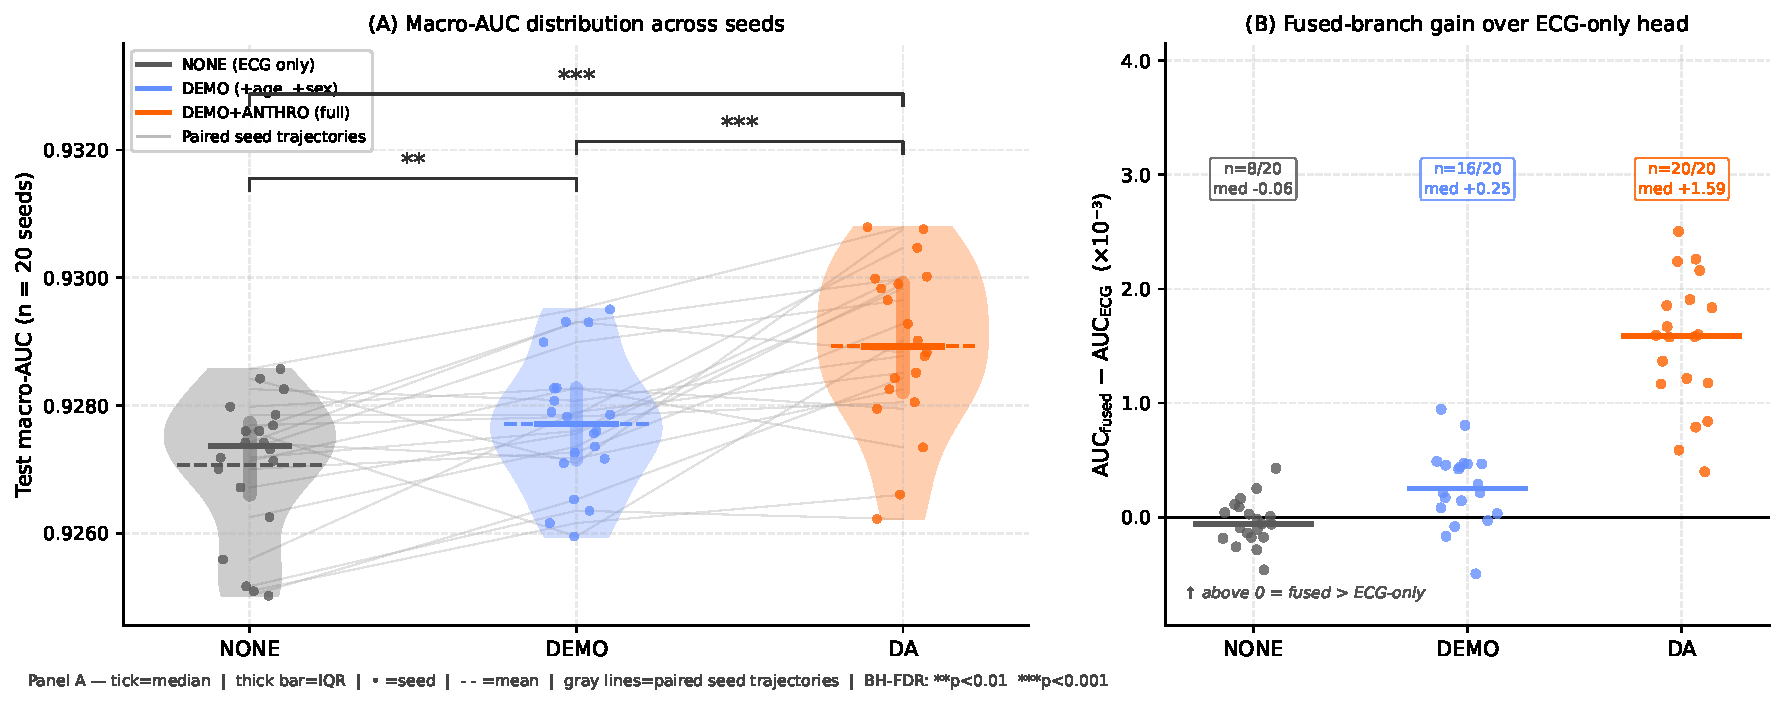
\includegraphics[width=\linewidth]{figures/fig6_seed_distribution.pdf}
\caption{Multi-seed reproducibility and architectural validation across \textbf{20 seeds}. \textbf{(A)}~Macro-AUC distribution per variant (violin = kernel density; thick bar = IQR; horizontal tick = median; dashed line = mean; dots = individual seeds; gray lines = paired seed trajectories). All three BH-FDR confirmatory brackets are shown: \texttt{demo}$-$\texttt{none} ($p_{\mathrm{BH}}{\approx}0.009$, $**$), \texttt{demo+anthro}$-$\texttt{demo} ($p_{\mathrm{BH}}{\approx}0.001$, $***$), \texttt{demo+anthro}$-$\texttt{none} ($p_{\mathrm{BH}}{<}0.001$, $***$); significance key: $**\,p_{\mathrm{BH}}{<}0.01$; $***\,p_{\mathrm{BH}}{<}0.001$. Gray paired trajectories show that \texttt{demo+anthro} exceeds \texttt{none} in 19 of 20 seeds and \texttt{demo} in 16 of 20. \textbf{(B)}~$\mathrm{AUC}_{\mathrm{fused}} - \mathrm{AUC}_{\mathrm{ECG}}$ per seed: the fused branch exceeds the ECG-only auxiliary head for all \textbf{20/20} seeds under \texttt{demo+anthro} (median $+0.0016$), confirming that the fusion mechanism captures the metadata signal at inference time. The gap is near-zero for \texttt{none} (8/20, median $-0.0001$) and intermediate for \texttt{demo} (16/20, median $+0.0003$). Note: the fused head is trained with both BCE and AUC surrogate losses while the ECG auxiliary head is trained with BCE only; this training asymmetry may also contribute to the fused--ECG gap, in addition to the metadata contribution.}
\label{fig:blend}
\end{figure}

% ---- Bibliography -----------------------------------------
\reftitle{References}
\externalbibliography{yes}
\bibliography{bibliography}

\end{document}
